%*******************************************************************************
%****************************** Fifth Chapter *********************************
%*******************************************************************************

\chapter{Cosmic Muon Tomography}

\ifpdf
    \graphicspath{{Chapter5/Figs/Raster/}{Chapter5/Figs/PDF/}{Chapter5/Figs/}}
\else
    \graphicspath{{Chapter5/Figs/Vector/}{Chapter5/Figs/}}
\fi

\section{Overview}
Cosmic $\mu$ tomography is split into two distinct types two sided and one sided. Two sided cosmic $\mu$ is preferred if it is feasible this is because both attenuation and scattering can be measured when using this technique. The effect of the cosmic $\mu$ scattering can be seen in figure \ref{fig:twoSidedCosmicMuonTomographySchults} the cosmic $\mu$ which travel through the dense object will scatter more than the cosmic $\mu$ that don't. By making coincident measurements of the cosmic $\mu$ it is possible to find vertices using this method. This method is extremely powerful but can only be used for smaller objects in most cases. 
\\\\ For larger objects one sided cosmic $\mu$ tomography has to be used. An example of what one sided cosmic muon tomography looks like can be seen in figure \ref{fig:oneSidedCosmicMuonExample} when there is an object that can attenuate cosmic $\mu$ then the number of cosmic $\mu$ will decrease in the direction of the object being imaged. This method cannot measure scattering or vertices however that is still sufficient in many cases such as the imaging done by the DIAPHANE collaboration seen in figure  \ref{fig:diaphaneStructualImaging}. Which uses 4 different locations to image the La Soufriere of Guadeloupe dome and measure the density for volcanic observations \cite{Marteau_2017}.
\begin{figure}[H]
 \centering
 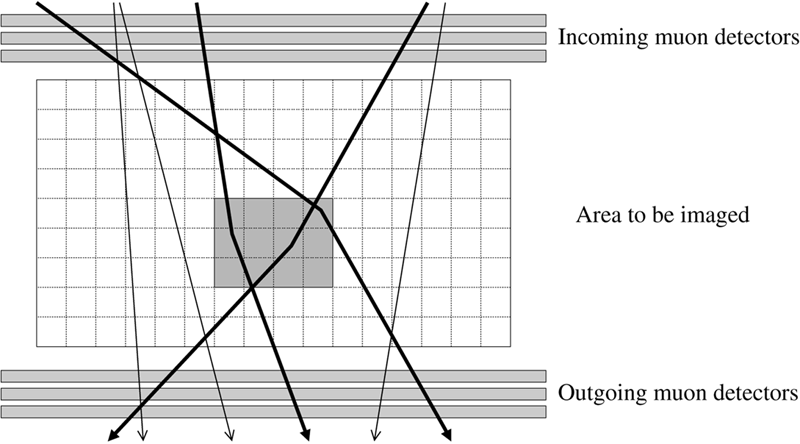
\includegraphics[width=0.8\linewidth]{Chapter5/Figs/Raster/twoSidedCosmicMuon_schults2007.png}
 \captionof{figure}{An side on view of two sided cosmic $\mu$ tomography the detectors are of similar size or larger than the object that is being measured in order to make coincided measurements using cosmic $\mu$ seen in the scattered (black) cosmic $\mu$ from \cite{schultz_2007}. }
 \label{fig:twoSidedCosmicMuonTomographySchults}
\end{figure}
 
 \begin{figure}[H]
 \centering
 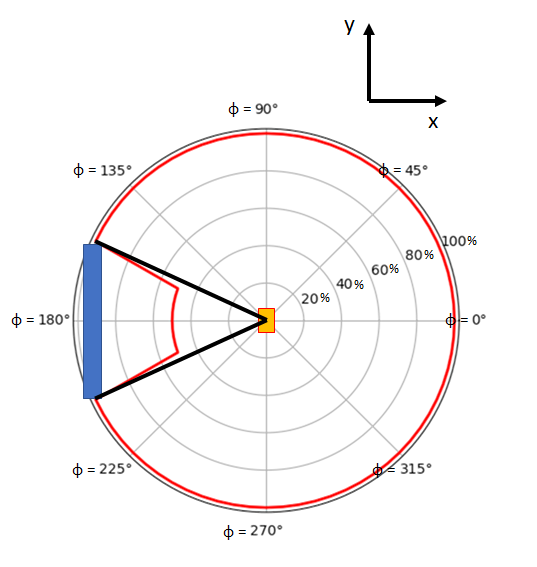
\includegraphics[width=0.7\linewidth]{Chapter5/Figs/wylfaRasterNew/TopDownCircularWallPlot.png}
 \captionof{figure}{.} 
 \label{fig:}
\end{figure}
 
 \begin{figure}[H]
 \centering
 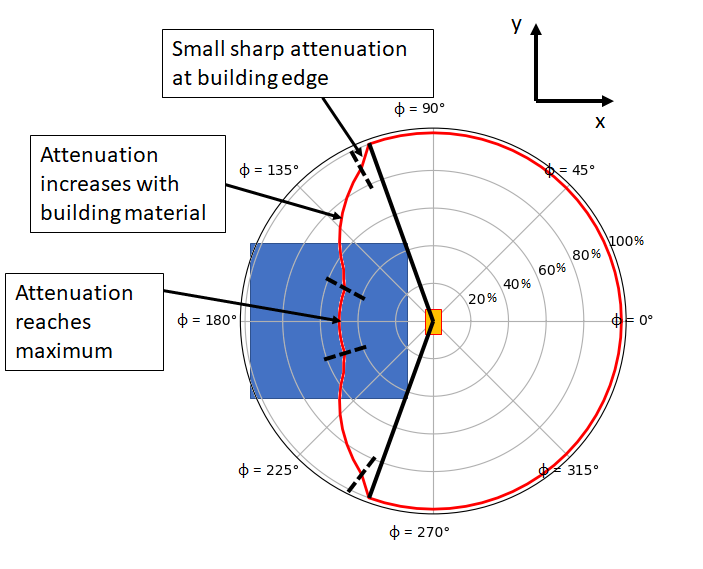
\includegraphics[width=0.9\linewidth]{Chapter5/Figs/wylfaRasterNew/TopDownCircularCubePlot.png}
 \captionof{figure}{.} 
 \label{fig:}
\end{figure}

 \begin{figure}[H]
 \centering
 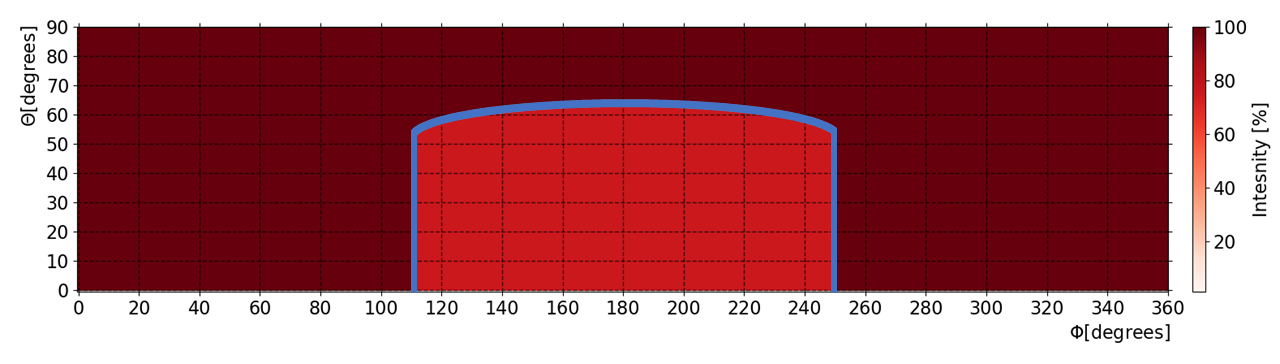
\includegraphics[width=0.9\linewidth]{Chapter5/Figs/wylfaRasterNew/thetaVsPhiExpectedCube.png}
 \captionof{figure}{.} 
 \label{fig:}
\end{figure}

%  \begin{figure}[H]
%  \centering
%  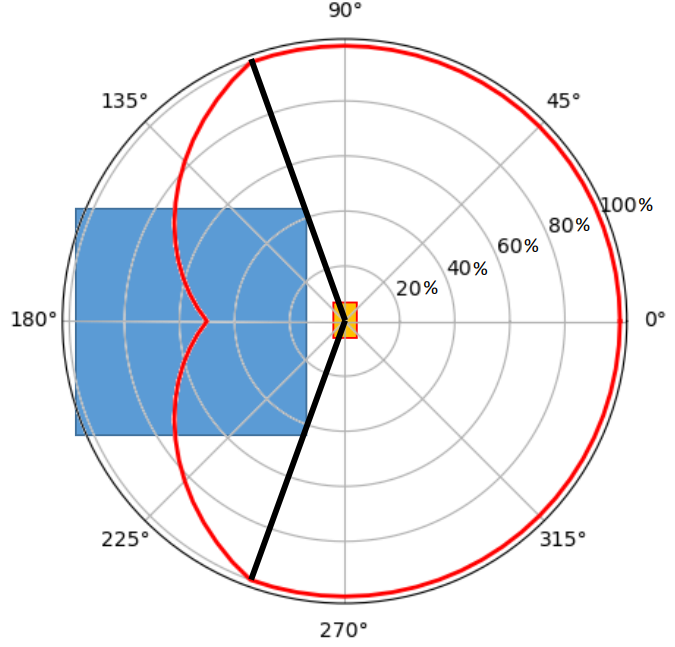
\includegraphics[width=0.6\linewidth]{Chapter5/Figs/Raster/oneSidedCosmicMuonExample.png}
%  \captionof{figure}{An example of what one sided cosmic $\mu$ tomography looks like from a top down view. When there is an object that attenuates $\mu$ significantly the percentage of $\mu$ detected decreases in the direction of the object.}
%  \label{fig:oneSidedCosmicMuonExample}
% \end{figure}
 
\begin{figure}[H]
 \centering
 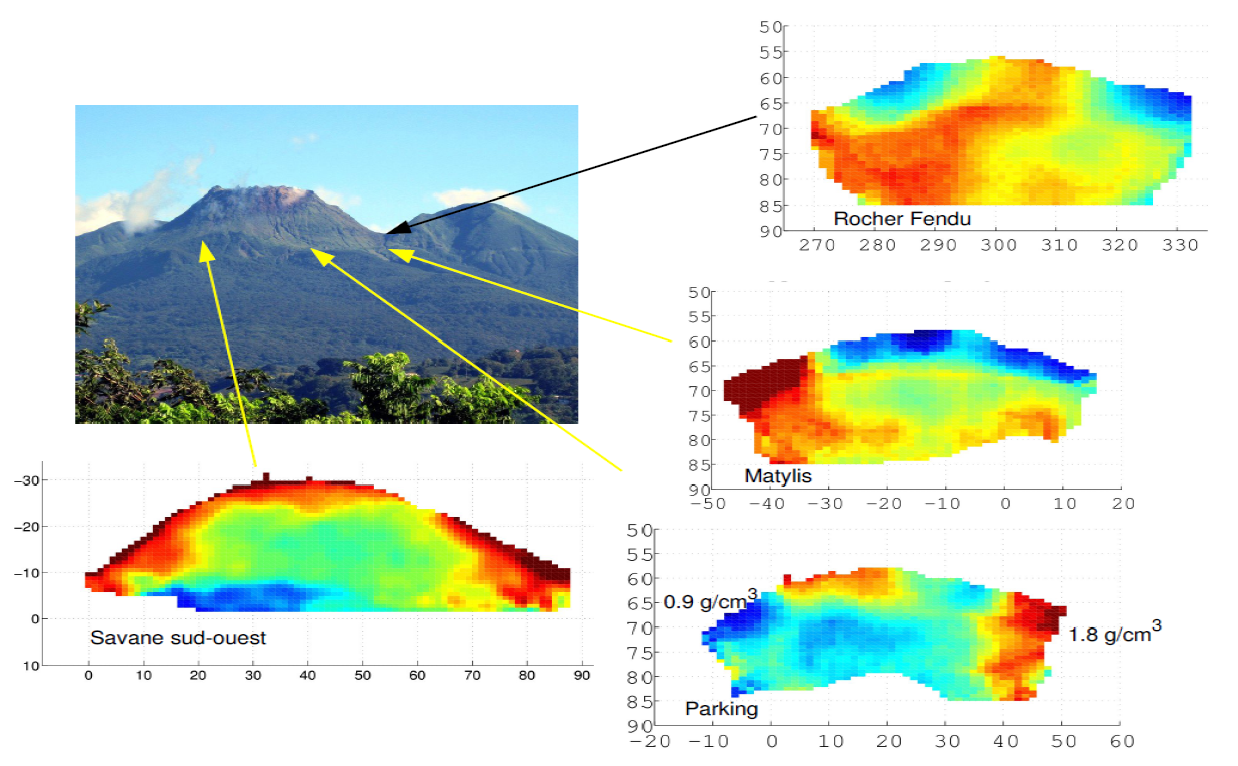
\includegraphics[width=1.0\linewidth]{Chapter5/Figs/Raster/diaphane_structuralImaging.png}
 \captionof{figure}{DIAPHANE structural imaging of the La Soufriere of Guadeloupe dome from 4 different acquisition sites around the dome. The blue areas are the less dense zones of the volcano. The red areas have the highest density. Average density extracted from all those images ranges from 1.6 to 1.8 g.cm$^{-3}$ from \cite{Marteau_2017}} %~can be used as a kind of place holder in latex
 \label{fig:diaphaneStructualImaging}
\end{figure}

\section{Deployment At Wylfa}\label{sec:deploymentAtWylfa}
The original prototype detector was deployed at the Wylfa Nuclear power station from 07-07-2014 to 25-02-2016 with data being taken continuously over that time period both with the reactor on and off with ibd measurements seen in figure \ref{fig:prototypeMeasumentFlux}. The placement of the detector in relation to the Wylfa reactor buildings can be seen in figure \ref{fig:wylfaTrace} the reactors were placed either end of the main reactor building in the centre of the cylindrical shaped ends. The overall shape of each of these buildings seen in figure \ref{fig:wylfaAir} causes the shape of the shadow to be quite different from what might be expected. The overall shadow in both $\theta$ and $\phi$ will therefore be an overlapping series of boxes rather than just one.   

\begin{figure}[H]
 \centering
 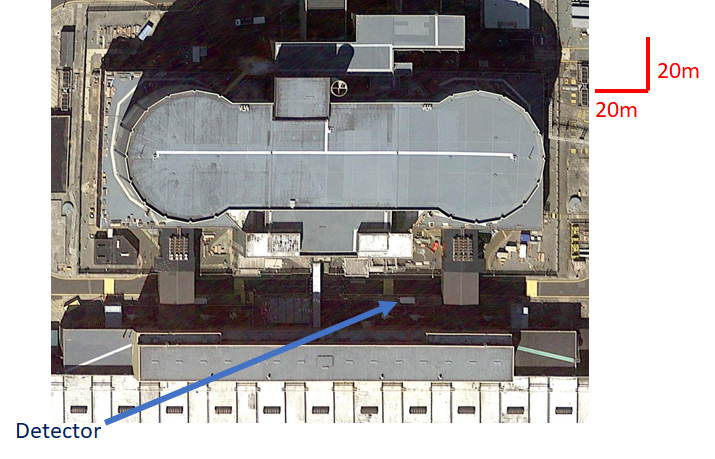
\includegraphics[width=0.7\linewidth]{Chapter5/Figs/wylfaRasterNew/DetectorPositionTopDown.png}
 \captionof{figure}{The position of the detector as shown by Google Earth.} %~can be used as a kind of place holder in latex
 \label{fig:DetectorPositionTopDown}
\end{figure}

\begin{figure}[H]
 \centering
 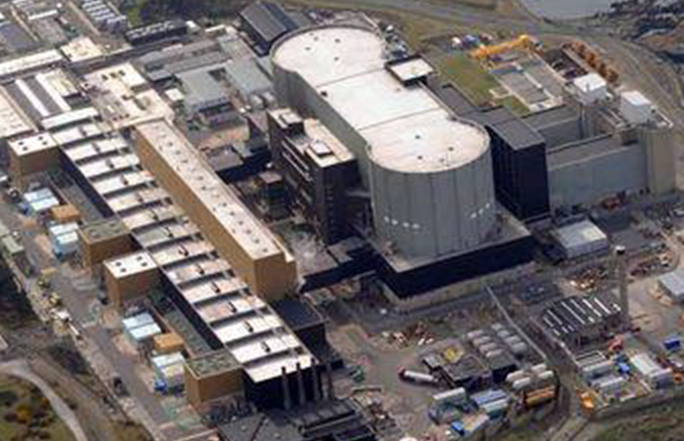
\includegraphics[width=0.7\linewidth]{Chapter5/Figs/Raster/wylfaArielView.png}
 \captionof{figure}{An aerial view of the Wylfa power station the main reactor building is the the shape of a "dog bone" the detector was placed in-between the turbine hall and reactor building.} %~can be used as a kind of place holder in latex
 \label{fig:wylfaAir}
\end{figure}

\section{Simulation Of Cosmic Muons}\label{sec:SimulationOfCosmics}

Before the data could be analysed a simulation of cosmic $\mu$ using a cosmic hemisphere was used in order to quantify segmentation effects and any other detector effects. These can be quite significant as seen in figures \ref{fig:phiGenVsRecoHem} and \ref{fig:cirPhiGenVsRecoHem} the reconstruction of our detector can be quite adversely effected by vertical events. If an event is vertical in one side of the detector then the other side will dominate as such it results in spikes at 0$^\circ$, 90$^\circ$, 180$^\circ$, 270$^\circ$. This bin migration is expected and due to its evenness should not have a significant effect on the shadows. 
\\\\ However this is only true with $\phi$, bin migration is significantly less pronounced in $\theta$ as seen in figure \ref{fig:thetaGenVsRecoHem}. Significant bin migration is is only seen in bins 0$^\circ$, 5$^\circ$, 80$^\circ$, 85$^\circ$, 90$^\circ$ but bins 10$^\circ$ -- 75$^\circ$ are accurately reconstructed. The large discrepancy in bin migration between $\theta$ and $\phi$ is due to the size of the segments in the VIDARR detector as they are 4\,cm wide by 1\,cm tall they are able to more accurately reconstruct information vertically than in any other direction. Which is useful for reconstructing vertical information such as the height of buildings. 
\begin{figure}[H]
 \centering
 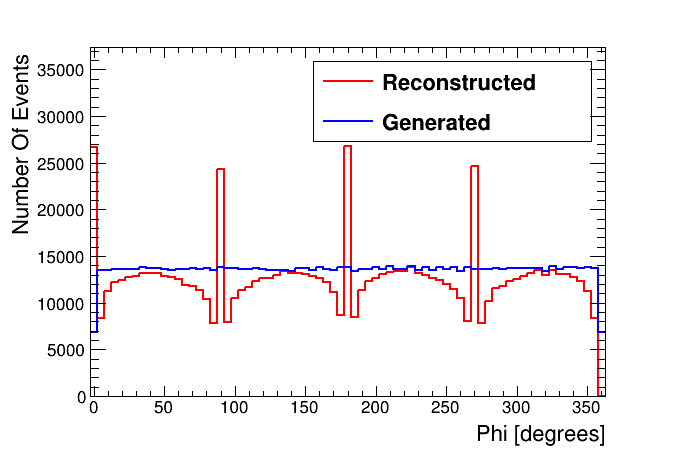
\includegraphics[width=0.8\linewidth]{Chapter5/Figs/Raster/hemispherePhiCompare.png}
 \captionof{figure}{Generated $\phi$ vs reconstructed $\phi$ with the online track fitter for a cosmic hemisphere distribution} %~can be used as a kind of place holder in latex
 \label{fig:phiGenVsRecoHem}
\end{figure}

\begin{figure}[H]
 \centering
 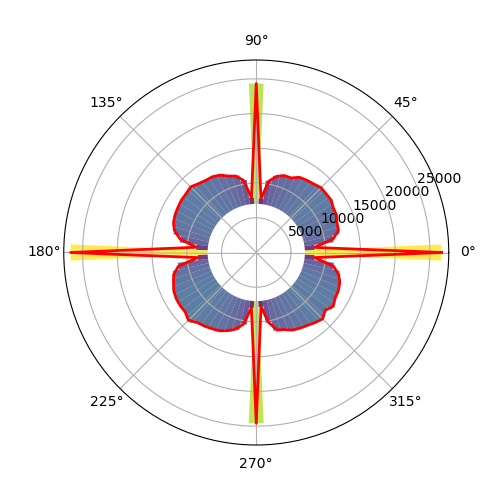
\includegraphics[width=0.6\linewidth]{Chapter5/Figs/Raster/cosmicSimpleHemNoDead_Ciruclarphi.png}
 \captionof{figure}{Circular plot of the reconstructed $\phi$ for a simulated cosmic hemisphere.} %~can be used as a kind of place holder in latex
 \label{fig:cirPhiGenVsRecoHem}
\end{figure}


\begin{figure}[H]
 \centering
 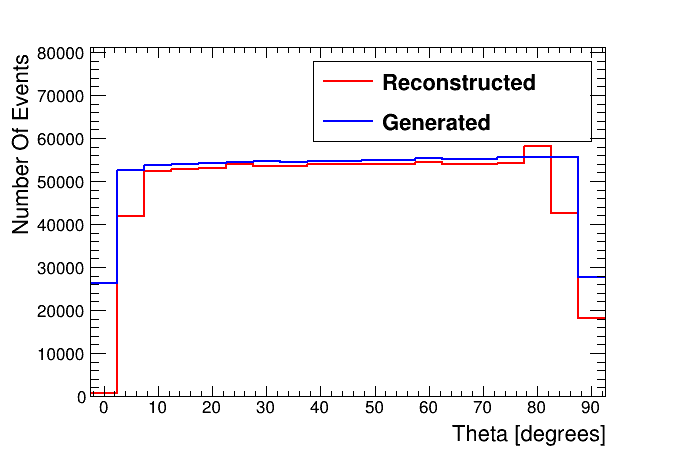
\includegraphics[width=0.8\linewidth]{Chapter5/Figs/Raster/hemisphereThetaCompare.png}
 \captionof{figure}{Generated $\theta$ vs reconstructed $\theta$ for a cosmic hemisphere distribution} %~can be used as a kind of place holder in latex
 \label{fig:thetaGenVsRecoHem}
\end{figure}

In order to quantify the effect of cosmic $\mu$ coming for every possible angle a cosmic hemisphere is simulated. The reconstruction of the cosmic hemisphere done by the tracker can be seen in figure \ref{fig:simulatedHemisphereDist}. The reconstruction artefacts shown in figures \ref{fig:phiGenVsRecoHem} and \ref{fig:thetaGenVsRecoHem} can also be seen to have a dependence on one another in figure \ref{fig:simulatedHemisphereDist}. Apart from the uncertainties introduced from segmentation there are no other uncertainties that are significant that are visible in \ref{fig:simulatedHemisphereDist}. However, this does not mean that that other uncertainties are not present just that the most noticeable uncertainty is due to the segmentation. 
\\\\ When trying to accurately reconstruct all the available cosmic $\mu$ there is no $\chi^2$ selection criteria. This is because many cosmic $\mu$ may shower when inside the detector and as a result may have a high $\chi^2$ but are still an accurate representation of cosmic $\mu$ direction. But a $\chi^2$ cut is effective when trying to accurately measure the $dE/dx$ as seen in figure \ref{fig:dedxGenVsRecoHem} showers produce many secondaries in the detector which when divided by the same length causes an increase in $dE/dx$ which is not justifiable. Therefore for positional reconstruction showers are kept but for online use where calibration is the goal showers are discarded.

\begin{figure}[H]
 \centering
 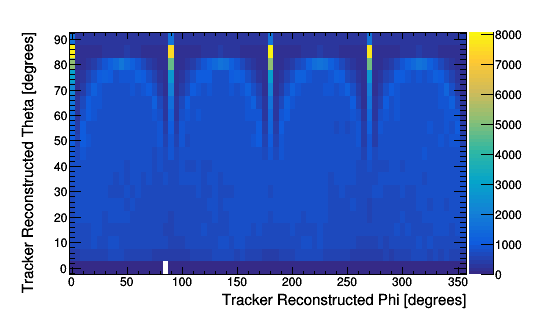
\includegraphics[width=0.8\linewidth]{Chapter5/Figs/Raster/pvsTFiduicalHemisphere.png}
 \captionof{figure}{Simulated cosmic hemisphere which has a flat distribution in $\theta$ from 0$^\circ$ to 90$^\circ$ and a flat distribution in $\phi$ from 0$^\circ$ to 360$^\circ$ which is then reconstructed using the online track fitter} %~can be used as a kind of place holder in latex
 \label{fig:simulatedHemisphereDist}
\end{figure}

\begin{figure}[H]
 \centering
 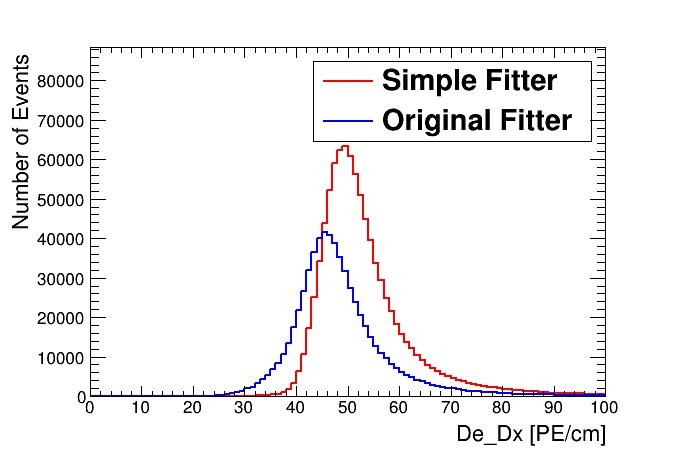
\includegraphics[width=0.8\linewidth]{Chapter5/Figs/Raster/dedxComarison.png}
 \captionof{figure}{\hl{need to add in generated de dx for this ploy} This is also more a show of the $\chi^2$/DOF effects the dE/dx and therefore how that may or may not be useful for online use.} %~can be used as a kind of place holder in latex
 \label{fig:dedxGenVsRecoHem}
\end{figure}

% \begin{figure}[H]
%  \centering
%  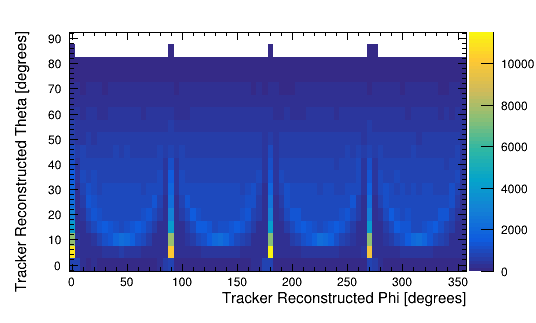
\includegraphics[width=0.8\linewidth]{Chapter5/Figs/Raster/simulatedNormalDistirbution.png}
%  \captionof{figure}{\hl{theta has been reversed now!!!} Simulated distribution with an ideally generated cosmic distribution.} %~can be used as a kind of place holder in latex
%  \label{fig:simulatedNormalDist}
% \end{figure}

\section{Reactor Shadow: Methodology} \label{sec:ReactorShadowMethodology}

\begin{figure}[H]
 \centering
 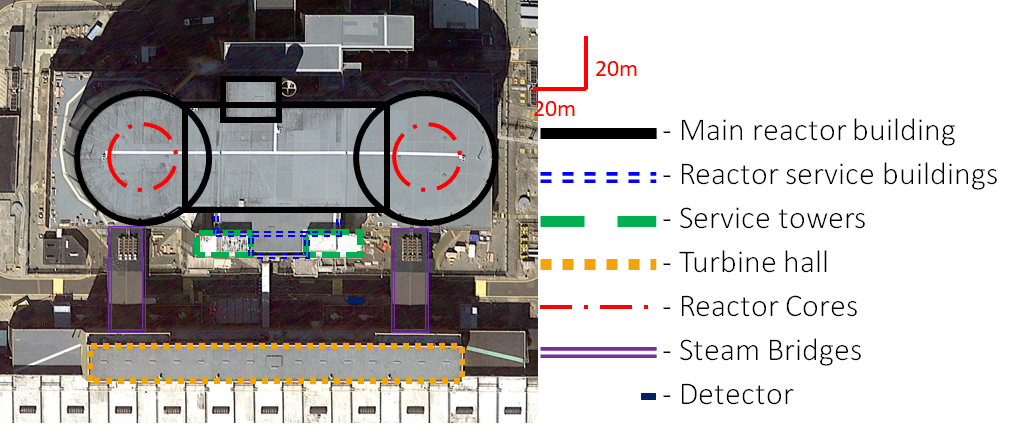
\includegraphics[width=\linewidth]{Chapter5/Figs/wylfaRasterNew/wylfaTraceStep1.png}
 \captionof{figure}{.} 
 \label{fig:}
\end{figure}

\begin{figure}[H]
 \centering
 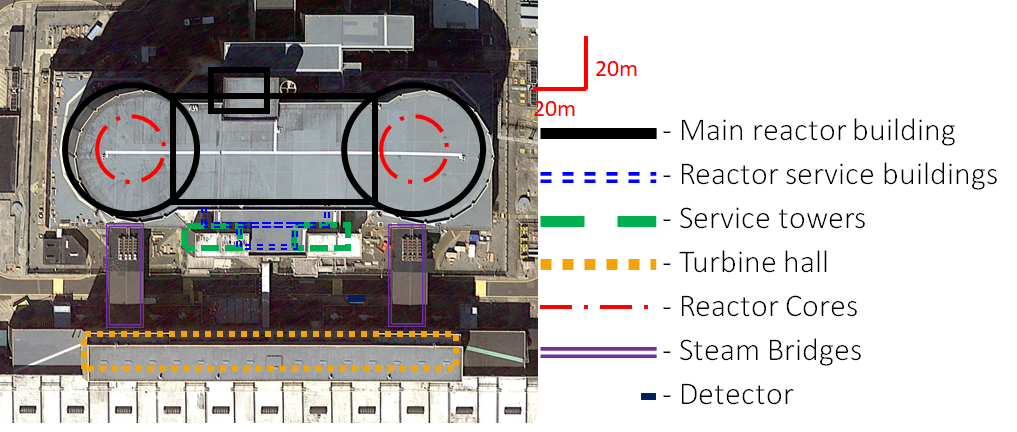
\includegraphics[width=\linewidth]{Chapter5/Figs/wylfaRasterNew/wylfaTraceStep2.png}
 \captionof{figure}{.} 
 \label{fig:}
\end{figure}

% \begin{figure}[H]
%  \centering
%  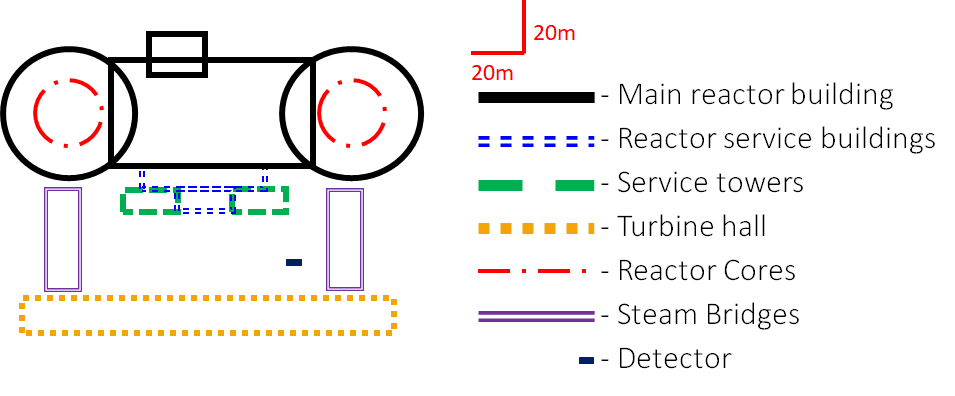
\includegraphics[width=\linewidth]{Chapter5/Figs/wylfaRasterNew/wylfaTraceStep3.png}
%  \captionof{figure}{.} 
%  \label{fig:}
% \end{figure}

\begin{figure}[H]
 \centering
 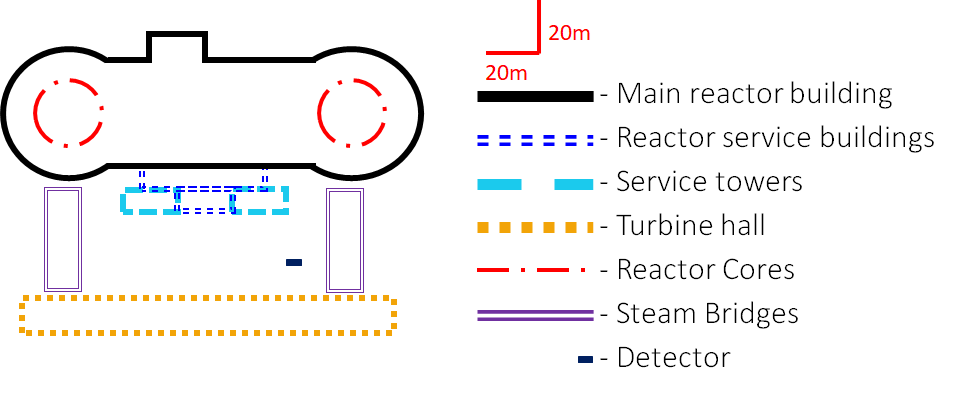
\includegraphics[width=\linewidth]{Chapter5/Figs/wylfaRasterNew/wylfaTraceStep4.png}
 \captionof{figure}{.} 
 \label{fig:}
\end{figure}

 \begin{figure}[H]
 \centering
 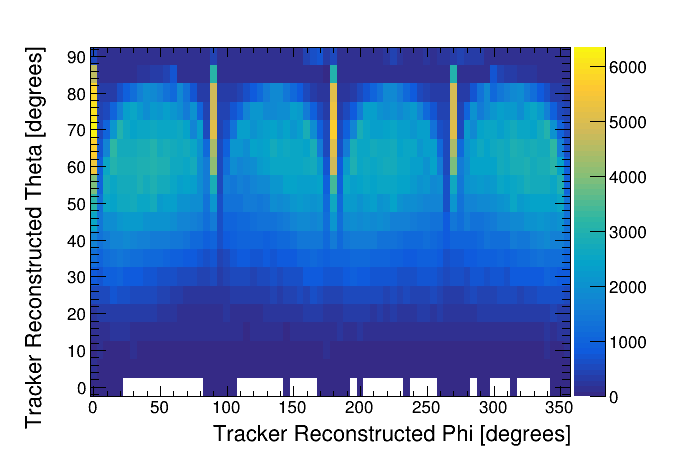
\includegraphics[width=0.7\linewidth]{Chapter5/Figs/Raster/pVsTWylfaReversed.png}
 \captionof{figure}{.} 
 \label{fig:}
\end{figure}

\begin{figure}[H]
 \centering
 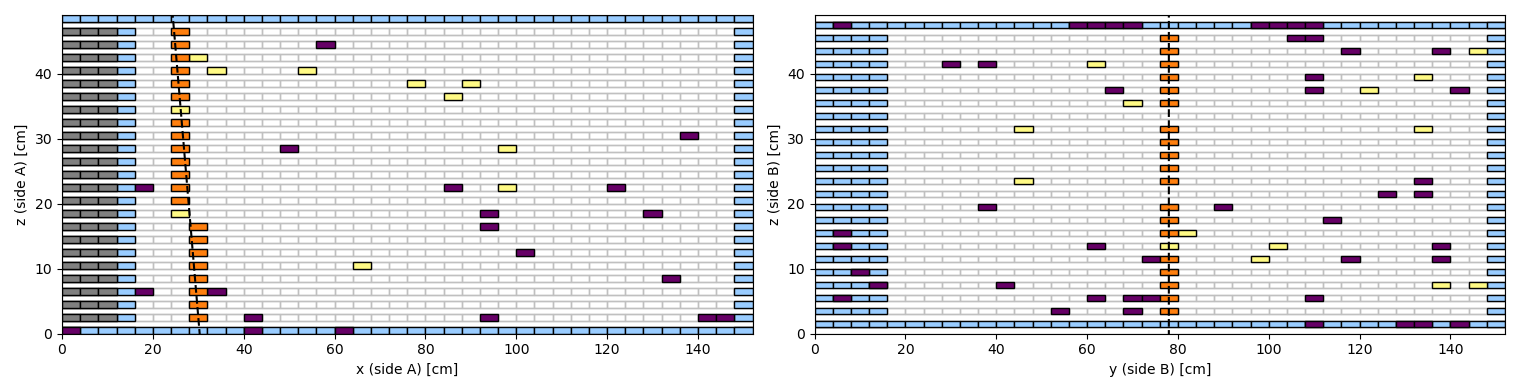
\includegraphics[width=\linewidth]{Chapter5/Figs/Raster/testEventNewScheme.png}
 \captionof{figure}{.} 
 \label{fig:}
\end{figure}

%  \begin{figure}[H]
%  \centering
%  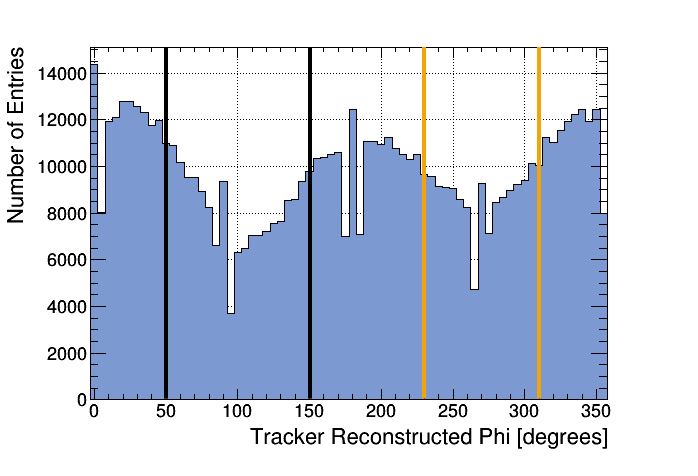
\includegraphics[width=0.7\linewidth]{Chapter5/Figs/wylfaRasterNew/LinearHist_theta_0-57.5_Deg.png}
%  \captionof{figure}{.} 
%  \label{fig:}
% \end{figure}

%  \begin{figure}[H]
%  \centering
%  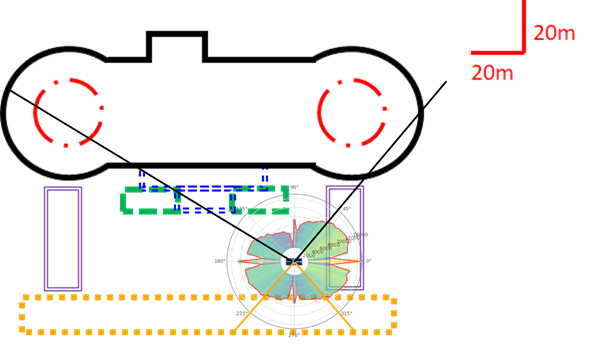
\includegraphics[width=\linewidth]{Chapter5/Figs/wylfaRasterNew/wylfaCircular0-57.5Deg_Overlay.png}
%  \captionof{figure}{.} 
%  \label{fig:}
% \end{figure}

\begin{figure}[H]
 \centering
 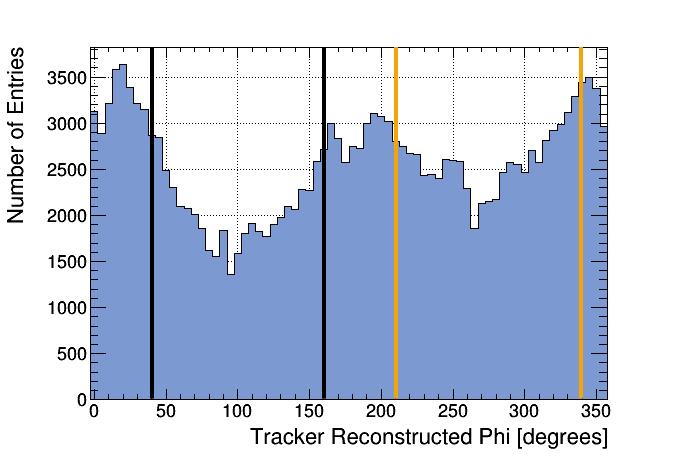
\includegraphics[width=0.7\linewidth]{Chapter5/Figs/wylfaRasterNew/LinearHist_theta_0-37.5_Deg.png}
 \captionof{figure}{.} 
 \label{fig:}
\end{figure}

 \begin{figure}[H]
 \centering
 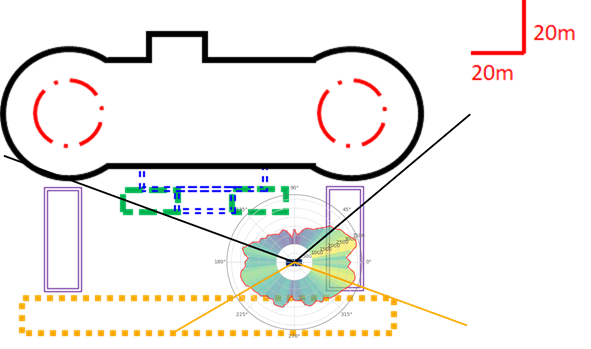
\includegraphics[width=\linewidth]{Chapter5/Figs/wylfaRasterNew/wylfaCircular0-37.5Deg_Overlay.png}
 \captionof{figure}{.} 
 \label{fig:}
\end{figure}

 \begin{figure}[H]
 \centering
 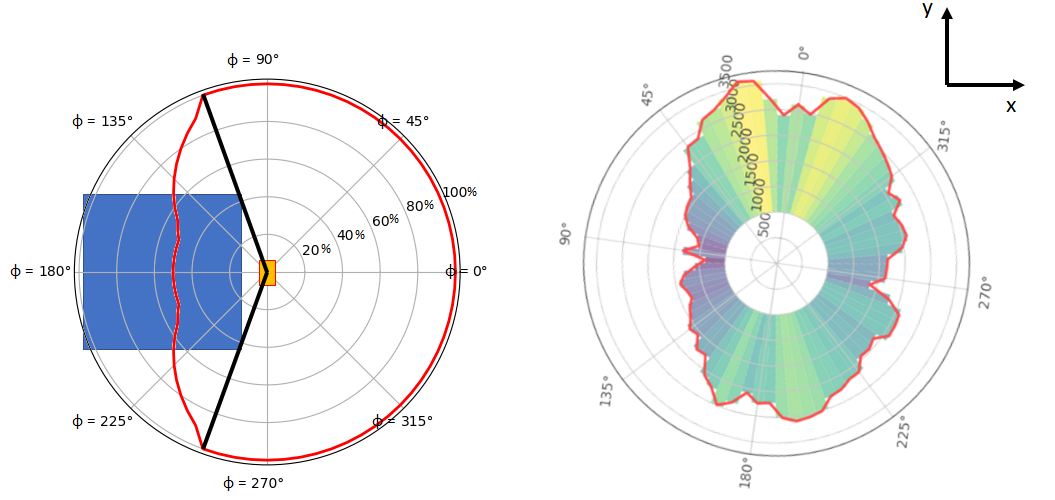
\includegraphics[width=\linewidth]{Chapter5/Figs/wylfaRasterNew/expectationVsRealityCircularPlot.png}
 \captionof{figure}{.} 
 \label{fig:}
\end{figure}

 \begin{figure}[H]
 \centering
 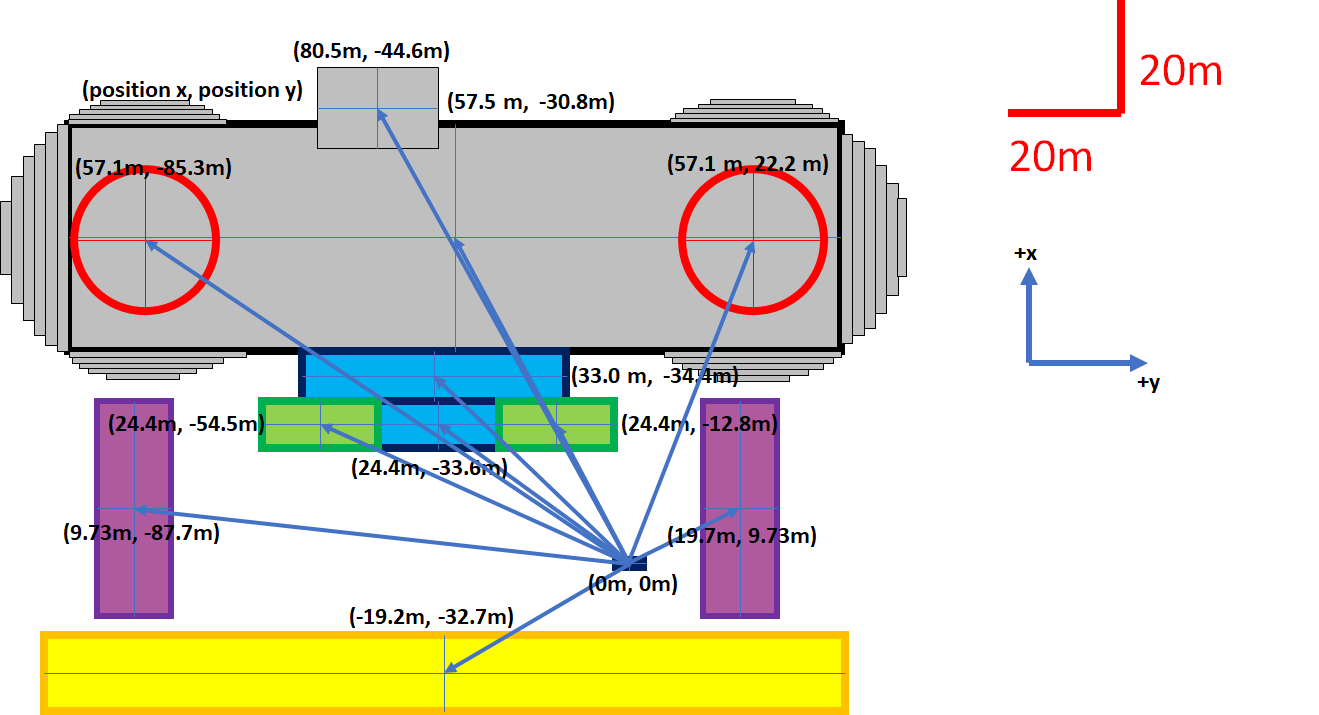
\includegraphics[width=\linewidth]{Chapter5/Figs/wylfaRasterNew/simulatedPositions.png}
 \captionof{figure}{.} 
 \label{fig:}
\end{figure}

\begin{figure}[H]
 \centering
 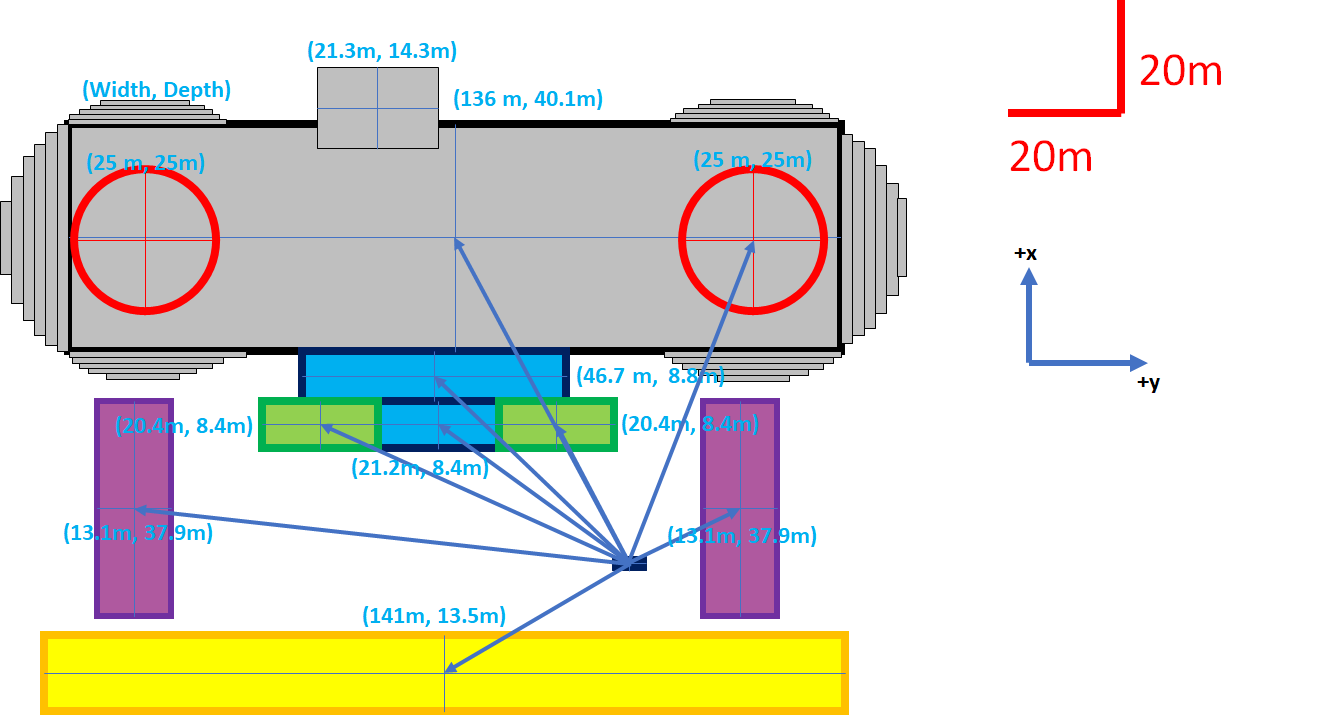
\includegraphics[width=\linewidth]{Chapter5/Figs/wylfaRasterNew/simulatedWidthsDepths.png}
 \captionof{figure}{.} 
 \label{fig:}
\end{figure}

\begin{figure}[H]
 \centering
 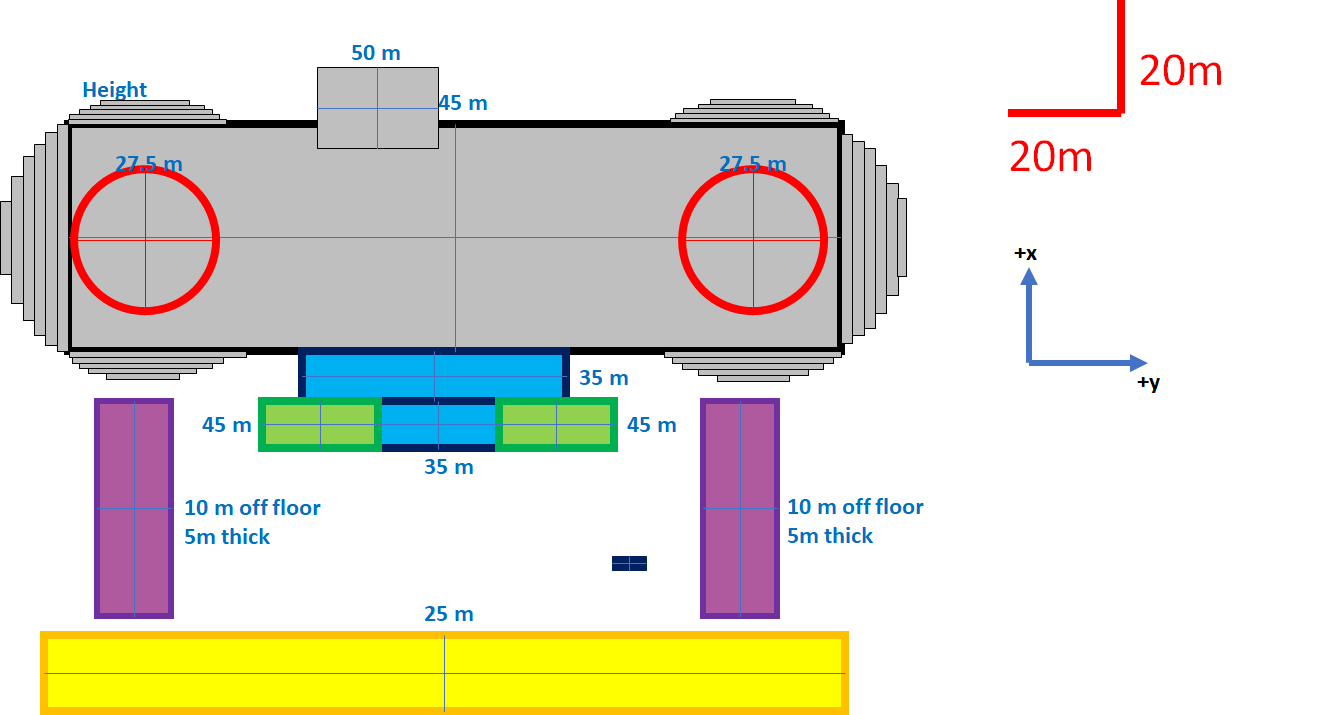
\includegraphics[width=\linewidth]{Chapter5/Figs/wylfaRasterNew/simulatedHeights.png}
 \captionof{figure}{.} 
 \label{fig:}
\end{figure}

\begin{figure}[H]
 \centering
 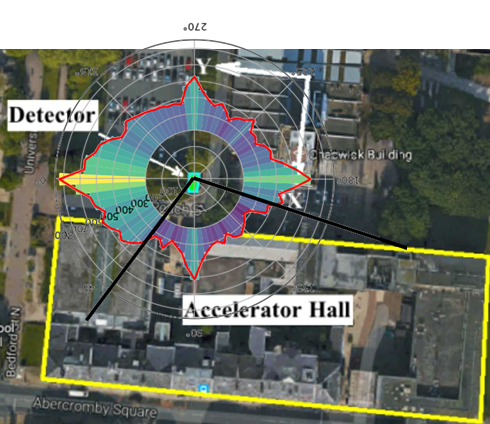
\includegraphics[width=\linewidth]{Chapter5/Figs/Raster/liverpoolShadows.png}
 \captionof{figure}{.} 
 \label{fig:}
\end{figure}

\begin{figure}[H]
 \centering
 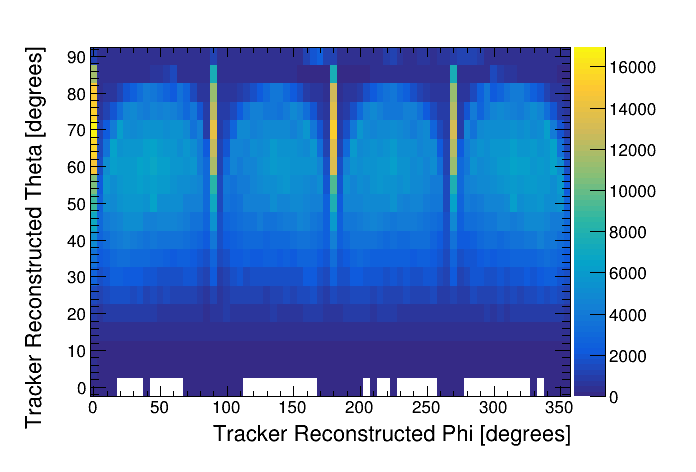
\includegraphics[width=0.7\linewidth]{Chapter5/Figs/Raster/pVsTLiverpoolReversed.png}
 \captionof{figure}{.} 
 \label{fig:}
\end{figure}

\begin{figure}[H]
\centering
\begin{subfigure}{.5\textwidth}
  \centering
  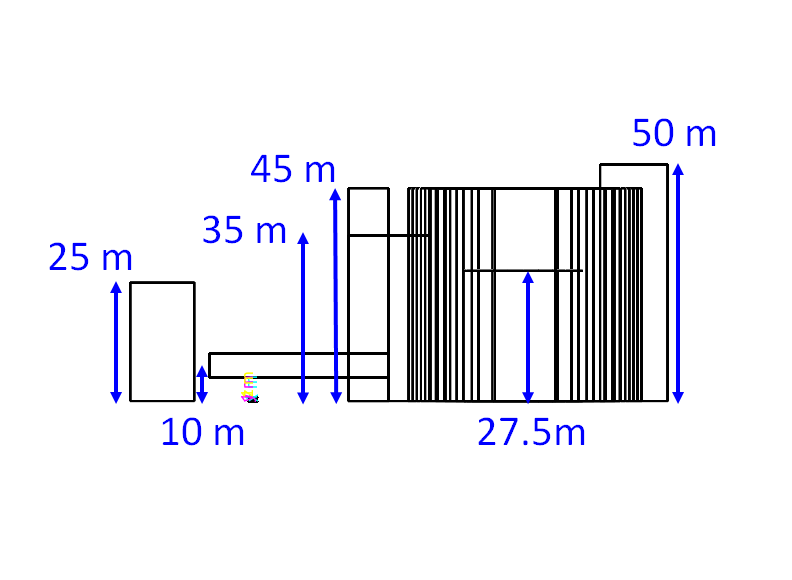
\includegraphics[width=\linewidth]{Chapter5/Figs/wylfaRasterNew/WylfaSimGeomSideOn.png}
  \captionsetup{width=.9\linewidth}
  \caption{.}
  \label{subFig:}
\end{subfigure}%
\begin{subfigure}{.5\textwidth}
  \centering
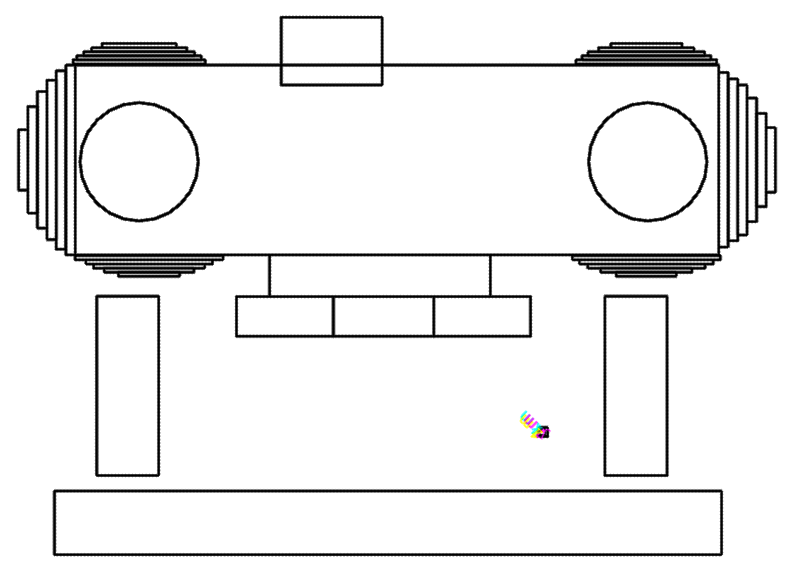
\includegraphics[width=\linewidth]{Chapter5/Figs/wylfaRasterNew/WylfaSimGeomTopDown.png}
  \captionsetup{width=.9\linewidth}
  \caption{.}
  \label{subFig:}
\end{subfigure}
\caption{.}
\label{fig:}
\end{figure}

\begin{figure}[H]
 \centering
 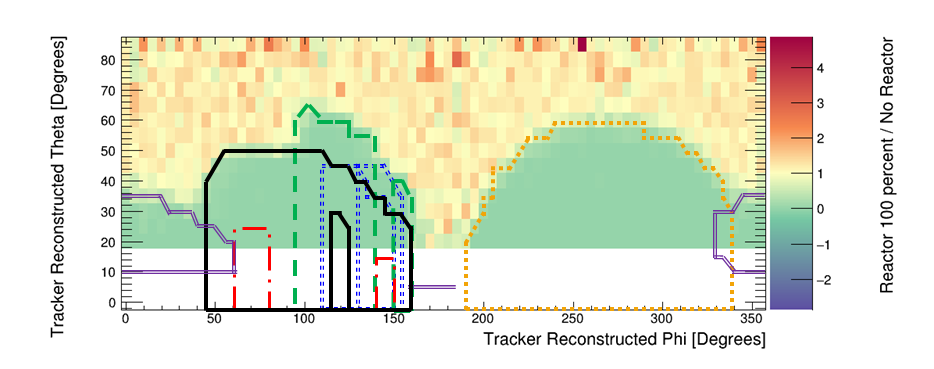
\includegraphics[width=\linewidth]{Chapter5/Figs/wylfaRasterNew/simulatedTrackerRecon.png}
 \captionof{figure}{.} 
 \label{fig:}
\end{figure}

\begin{figure}[H]
 \centering
 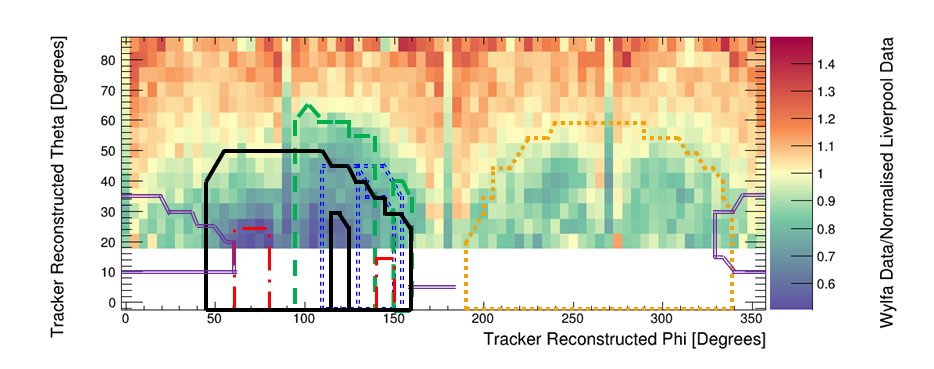
\includegraphics[width=\linewidth]{Chapter5/Figs/wylfaRasterNew/measuredTrackerRecon.png}
 \captionof{figure}{.} 
 \label{fig:}
\end{figure}

\begin{figure}[H]
 \centering
 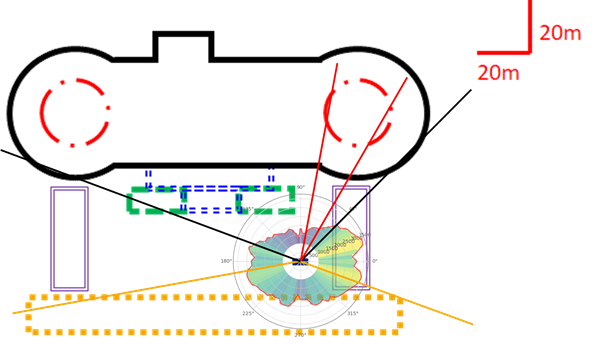
\includegraphics[width=\linewidth]{Chapter5/Figs/wylfaRasterNew/wylfaCircular0-37.5Deg_Overlay_Updated.png}
 \captionof{figure}{.} 
 \label{fig:}
\end{figure}

% In order to find the approximate position of detector at the Wylfa site Google Maps was used as the detector's container was large enough to be seen by the Google Maps satellite. The initial step can be seen in figure \ref{fig:wylfaTraceStep0}. Once the detector position has been identified a rough trace of the buildings is then performed with basic shapes seen in figure \ref{fig:wylfaTraceStep1}. However because the site buildings are taller than the detector by quite a significant margin the base position of the buildings does not match the top position of the buildings seen in the google maps. In figure \ref{fig:wylfaTraceStep2} key areas of the site buildings are used as anchor points to so that the base of the buildings is more accurately represented. Finally the background and any connecting lines are removed in figure \ref{fig:wylfaTraceStep4} which shows the final Wylfa trace.  

% \begin{figure}[H]
%  \centering
%  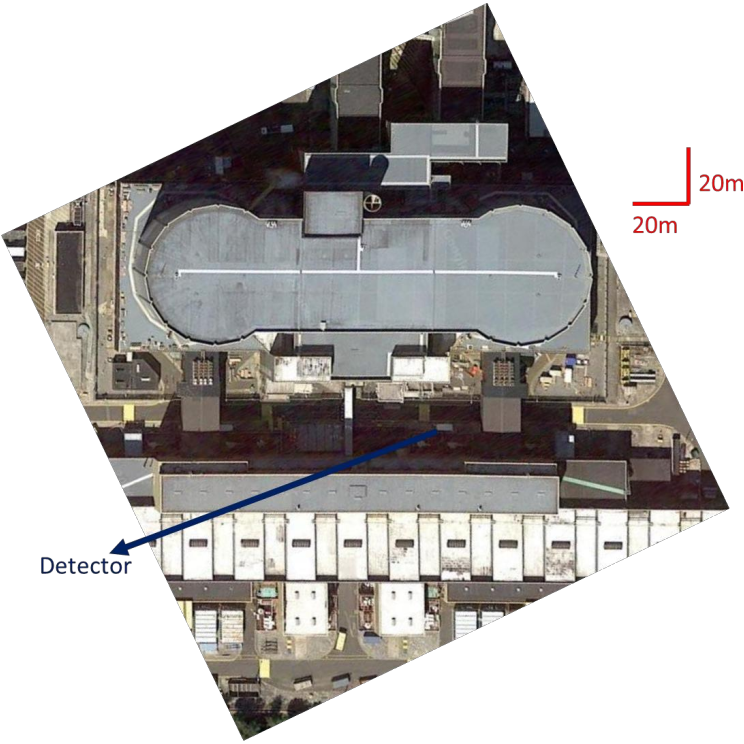
\includegraphics[width=\linewidth]{Chapter5/Figs/Raster/wylfaTraceStep0.png}
%  \captionof{figure}{The detector at the Wylfa reactor site.} 
%  \label{fig:wylfaTraceStep0}
% \end{figure}

% \begin{figure}[H]
%  \centering
%  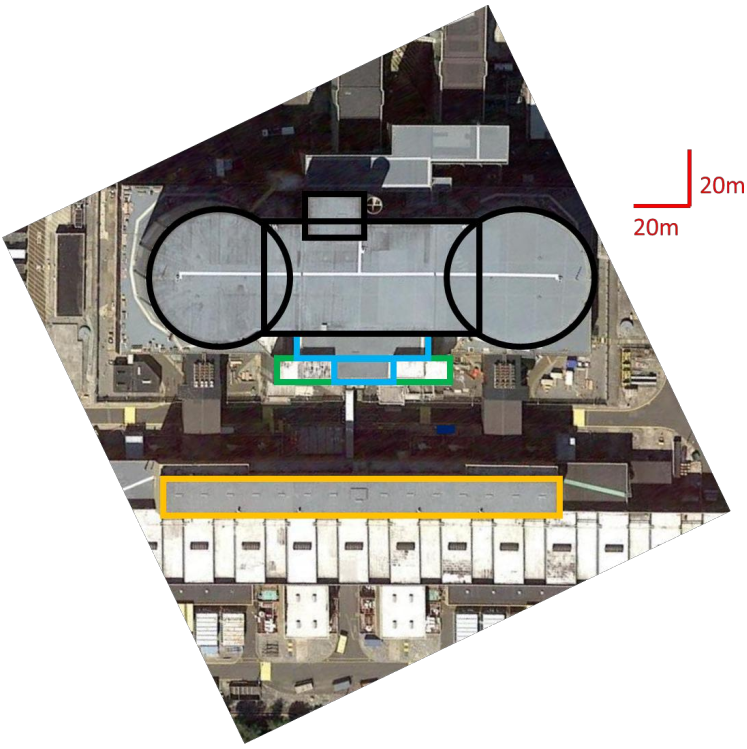
\includegraphics[width=\linewidth]{Chapter5/Figs/Raster/wylfaTraceStep1.png}
%  \captionof{figure}{Basic shapes are overlaid on top of the detector and site buildings.} 
%  \label{fig:wylfaTraceStep1}
% \end{figure}

% \begin{figure}[H]
%  \centering
%  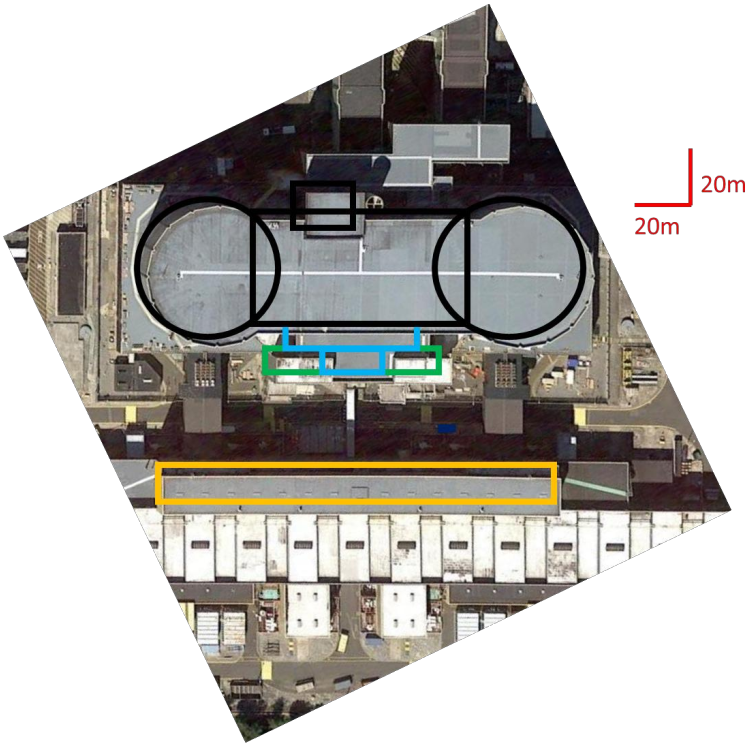
\includegraphics[width=\linewidth]{Chapter5/Figs/Raster/wylfaTraceStep2.png}
%  \captionof{figure}{Anchor points are used to offset the tall site buildings closer to the base of the buildings. This is done to take into account the angle of the google maps satellite.} 
%  \label{fig:wylfaTraceStep2}
% \end{figure}

% \begin{figure}[H]
%  \centering
%  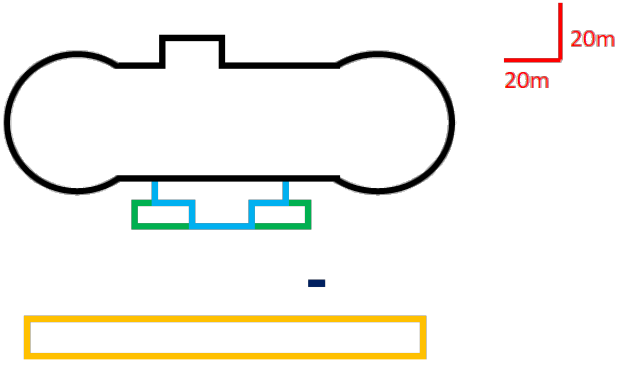
\includegraphics[width=\linewidth]{Chapter5/Figs/Raster/wylfaTraceStep4.png}
%  \captionof{figure}{Finally the background of the reactor site is removed and we are left with a trace of the reactor site.} 
%  \label{fig:wylfaTraceStep4}
% \end{figure}

% The cosmic $\mu$ tracker has several steps. First if fewer than 8 bars are hit above 0.7\,MeV the event is discarded. Then if either side has less than 4 hits > 0.7\,MeV the event is discarded. Then the top and bottom hit is found for each side of the detector from this a basic approximation of the gradient is found. This provides a starting point for the fitter on each side, this leads to the initial fit where all of the events above the 0.7\,MeV threshold are fitted, this is preferred over clustering as it includes low angled $\theta$ cosmic $\mu$ that clustering often removes. Then any hits that are 2 bars away from the track are discarded, and any lone hits that are 8 bars away from any other hits are also removed then the second fit is applied. Then any hits within one bar of the fitted track are then re-accepted as part of the track. Any lone hits to within a radius of 4 bars from the track are once again removed. This then leads to the third and final fit, which is very fast as the approximation by the second fit is usually quite close to third fit. Then any track which has less than 4 hits per side is then rejected. Finally if 50\,\% of the track energy is missing in either side the event is also removed, this is because under such circumstances it is likely that a second cosmic event is inside the detector or a shower has produced multiple tracks. In figure \ref{fig:3000ExampleEvent} it can be seen that even with a large number of noise hits ($\sim$ 10 noise hits per side) the fitter has still accurately reconstructed the event. 
 
% \begin{figure}[H]
%  \centering
%  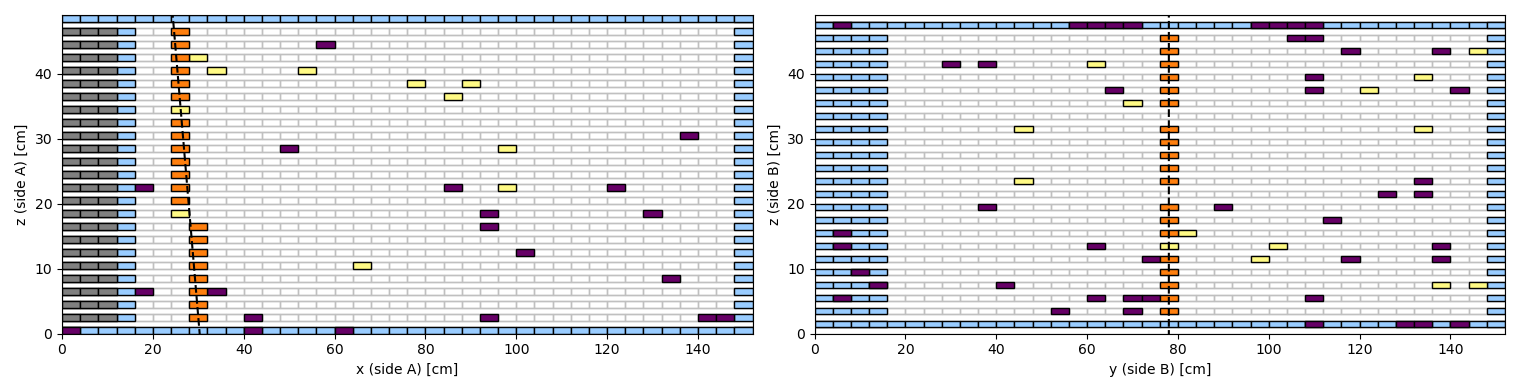
\includegraphics[width=\linewidth]{Chapter5/Figs/Raster/testEventNewScheme.png}
%  \captionof{figure}{An example event from the Wylfa deployment the cosmic enters through the top of the detector and exits through the bottom. The signal that the tracker has identified is shown in orange. The hits the tracker discards are shown in yellow. The un-instrumented block on side A is shown in grey. The dead channels are shown in dark purple. The channels removed for fiducial purposes are shown in light blue.} 
%  \label{fig:3000ExampleEvent}
% \end{figure}

% Using this fitter the data from both the 2014 -- 2015 Wylfa deployment, figure \ref{fig:pVsTWylfaReversed}, and the 2015 -- 2018 deployment at Liverpool, figure \ref{fig:pVsTLiverpoolReversed}, can be analysed for tomographic purposes. Both of these data sets have shadows in them, the shadows in the Liverpool data set are significantly fainter than the shadows in the Wylfa data as the buildings at Wylfa are mostly comprised of concrete where as the buildings at Liverpool are mostly comprised of brick, glass, and steel. In the Liverpool data set the shadows are only visible at very shallow angles of $\theta$ due to the difference in building densities. At Liverpool whilst other buildings are visible in the data set the old accelerator hall is the most visible component which is highlighted in figure \ref{fig:liverpoolCirShadows}. However these shadows are only visible from 0$^{\circ}$ $\theta$ -- 17.5$^{\circ}$ $\theta$, at angles higher than 17.5 $^{\circ}$ $\theta$ the shadows are too faint. 
% \begin{figure}[H]
%  \centering
%  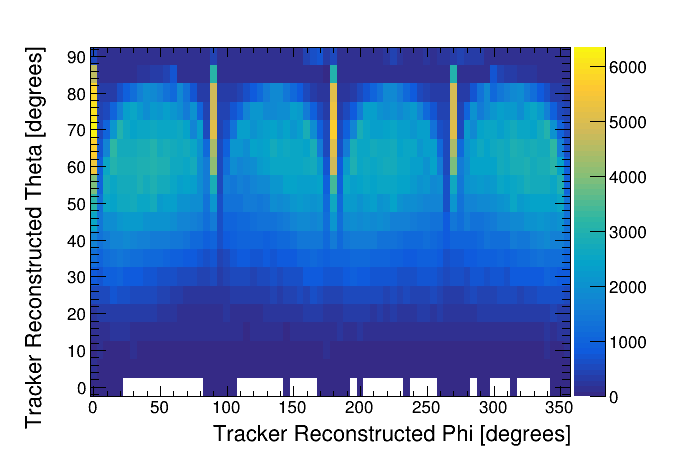
\includegraphics[width=0.8\linewidth]{Chapter5/Figs/Raster/pVsTWylfaReversed.png}
%  \captionof{figure}{Measured $\theta$ and $\phi$ from the cosmic muons from the Wylfa deployment, the reactor is at $\sim$ 90$^{\circ}$. The turbine hall is at $\sim$ 270$^{\circ}$.} 
%  \label{fig:pVsTWylfaReversed}
% \end{figure}

% \begin{figure}[H]
%  \centering
%  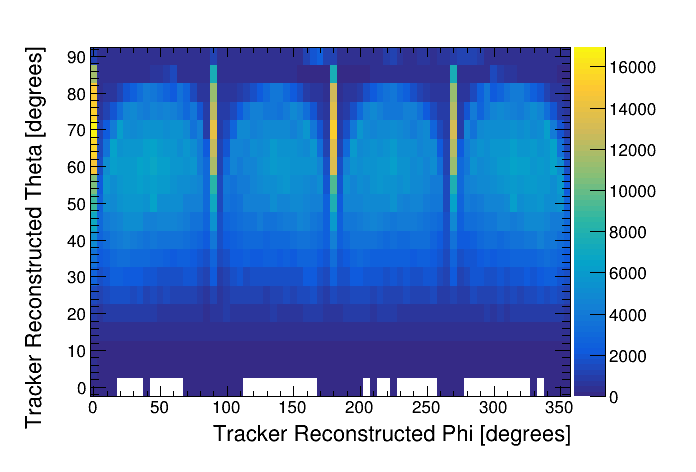
\includegraphics[width=0.8\linewidth]{Chapter5/Figs/Raster/pVsTLiverpoolReversed.png}
%  \captionof{figure}{Measured $\theta$ and $\phi$ from the cosmic muons from the Liverpool deployment.} 
%  \label{fig:pVsTLiverpoolReversed}
% \end{figure}

% \begin{figure}[H]
%  \centering
%  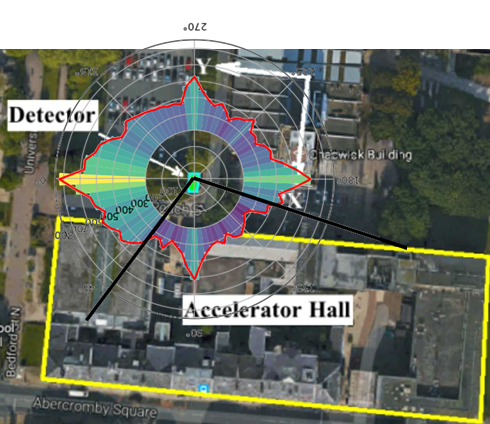
\includegraphics[width=0.8\linewidth]{Chapter5/Figs/Raster/liverpoolShadows.png}
%  \captionof{figure}{Measured $\theta$ and $\phi$ from the cosmic muons from the Liverpool deployment shown with the map of Liverpool in the background. The major dip at highlighted by the black lines is due to the accelerator hall at Liverpool.} 
%  \label{fig:liverpoolCirShadows}
% \end{figure}

% The shadows in the Wylfa data are much clearer, seen in figures \ref{fig:WylfaSlice0-57.5} and \ref{fig:wylfaTraceAbove32.5} shows $\phi$ from 0$^{\circ}$ $\theta$ -- 57.5$^{\circ}$ $\theta$ the shadows are clearly visible from both the turbine hall highlighted in-between the orange lines and the reactor buildings shown in-between the black lines. The shape however does not accurately represent the size of the reactor footprint or the width of the turbine hall. This is due to the angles of cosmic $\mu$ that are being attenuated by the buildings. In order to accurately quantify the width of the reactor building cosmic $\mu$ from lower angles must be considered in figures \ref{fig:WylfaSlice0-37.5} and \ref{fig:wylfaTraceAbove52.5}  show $\phi$ from 0$^{\circ}$ $\theta$ -- 37.5$^{\circ}$ $\theta$ this now gives a much more accurate estimate for the size of the reactor building and $phi$. The size of the turbine hall in $\phi$ is less accurate due to the corrugated steel the turbine hall is constructed with, this means the far edge of the turbine hall is hard to discern which can be seen in figure \ref{fig:wylfaTraceAbove52.5}.

% \begin{figure}[H]
% \centering
% \begin{subfigure}{.5\textwidth}
%   \centering
%   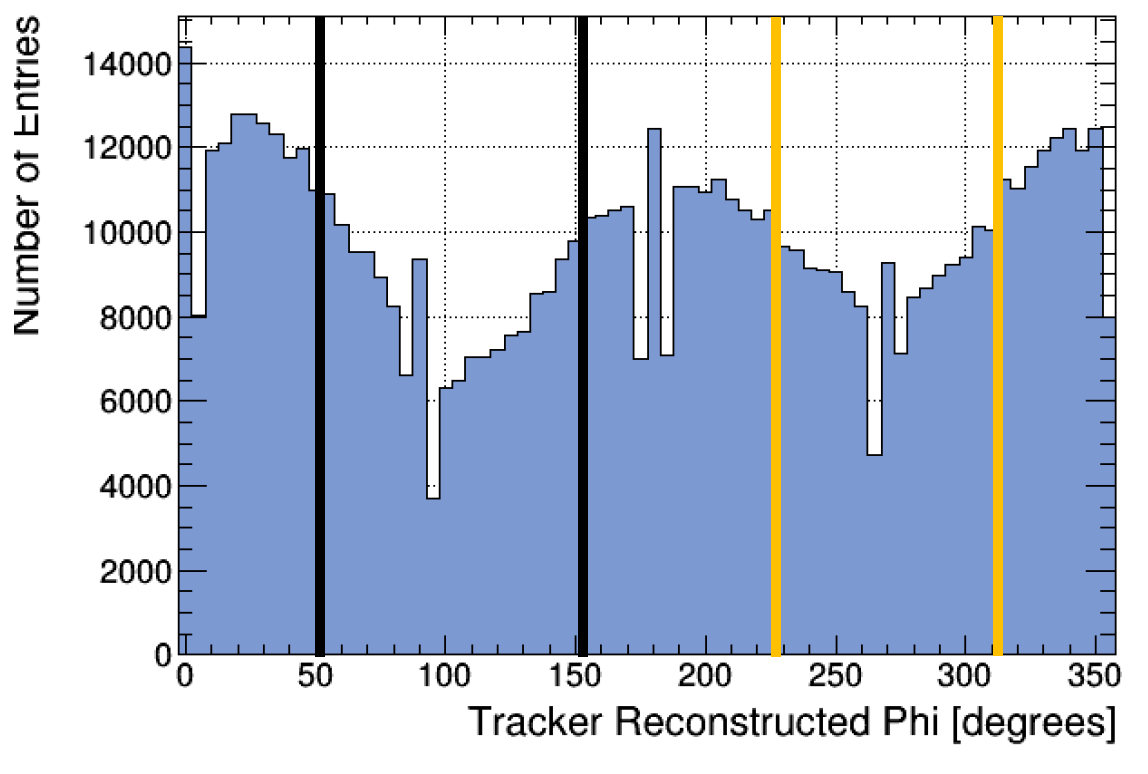
\includegraphics[width=\linewidth]{Chapter5/Figs/Raster/linReversedWylfaSlice0-57.5.png}
%   \captionsetup{width=.9\linewidth}
%   \caption{Linear histogram showing the dips in the shadows from the shadows of the reactor buildings and turbine halls.}
%   \label{subFig:linReversedWylfaSlice0-57.5}
% \end{subfigure}%
% \begin{subfigure}{.5\textwidth}
%   \centering
%   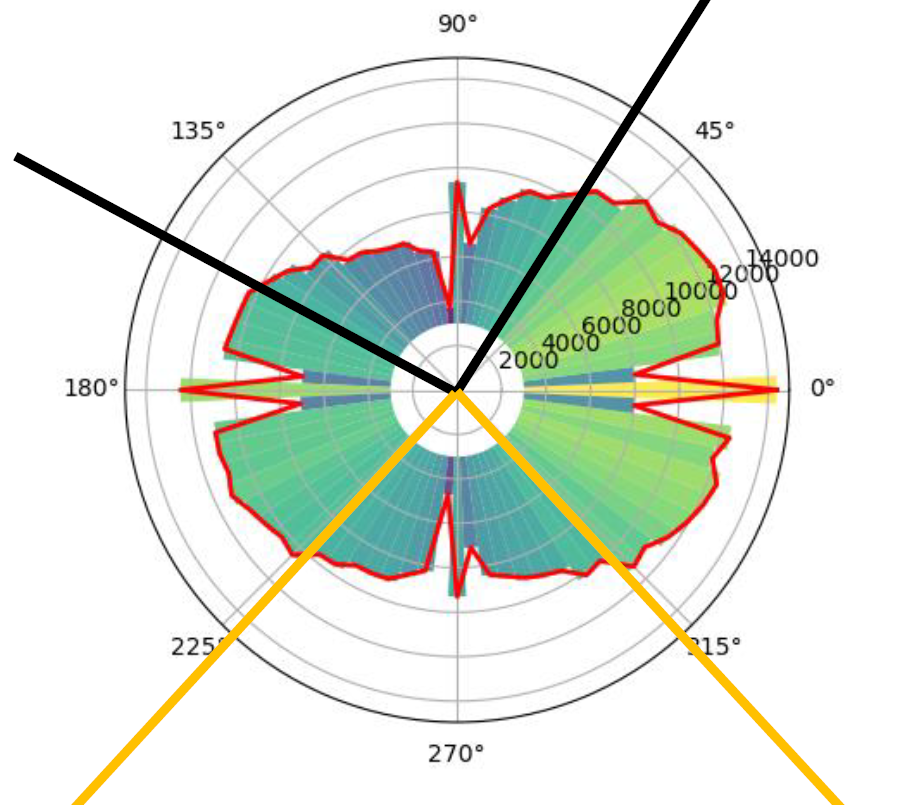
\includegraphics[width=0.765\linewidth]{Chapter5/Figs/Raster/cirReversedWylfaSlice0-57.5.png}
%   \captionsetup{width=.9\linewidth}
%   \caption{Circular histogram showing the dips in the shadows from the shadows of the reactor buildings and turbine halls.}
%   \label{subFig:linReversedWylfaSlice0-57.5}
% \end{subfigure}
% \caption{Histograms showing how the shadows of the reactor buildings and the turbine hall are cast on to the detector from $\theta$ of 0$^\circ$ to 57.5$^\circ$. The Reactor buildings are shown in-between the black lines the turbine hall is shown in-between the orange lines.}
% \label{fig:WylfaSlice0-57.5}
% \end{figure}

% \begin{figure}[H]
%  \centering
%  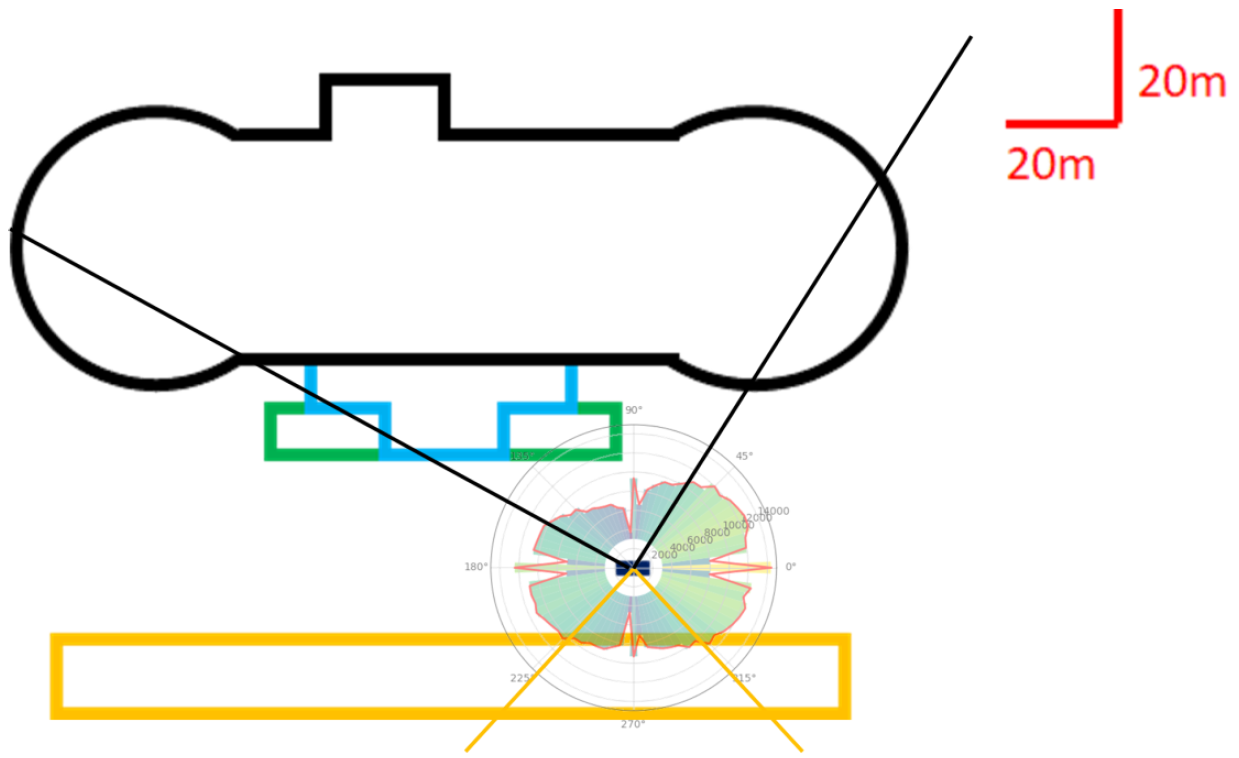
\includegraphics[width=\linewidth]{Chapter5/Figs/Raster/cirOverlayReversedWylfaSlice0-57.5.png}
%  \captionof{figure}{The circular distribution of the $\phi$ from a $\theta$ of 0$^\circ$ - 57.5$^\circ$ traced over from google maps and then compared with the documentation given by Wylfa reactor operators. The tower closest to the detector is dominating the distribution of the shadow.} %~can be used as a kind of place holder in latex
%  \label{fig:wylfaTraceAbove32.5}
% \end{figure}

% \begin{figure}[H]
% \centering
% \begin{subfigure}{.5\textwidth}
%   \centering
%   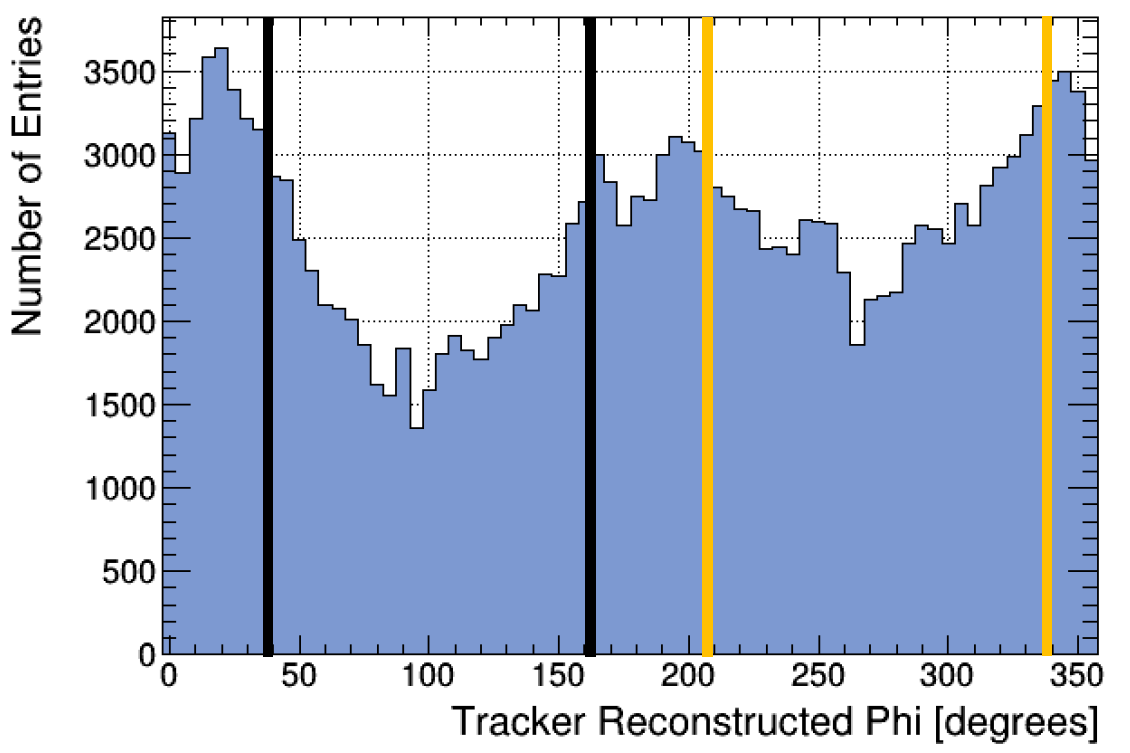
\includegraphics[width=\linewidth]{Chapter5/Figs/Raster/linReversedWylfaSlice0-37.5.png}
%   \captionsetup{width=.9\linewidth}
%   \caption{Linear histogram showing the dips in the shadows from the shadows of the reactor buildings and turbine halls.}
%   \label{subFig:linReversedWylfaSlice0-37.5}
% \end{subfigure}%
% \begin{subfigure}{.5\textwidth}
%   \centering
%   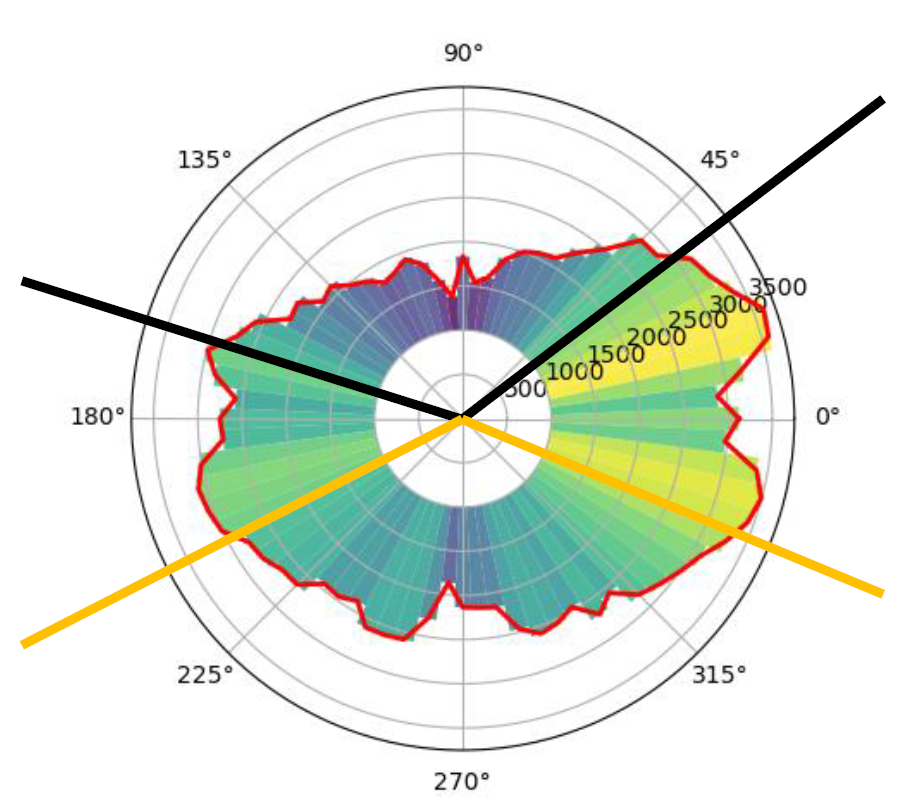
\includegraphics[width=0.765\linewidth]{Chapter5/Figs/Raster/cirReversedWylfaSlice0-37.5.png}
%   \captionsetup{width=.9\linewidth}
%   \caption{Circular histogram showing the dips in the shadows from the shadows of the reactor buildings and turbine halls.}
%   \label{subFig:cirReversedWylfaSlice0-37.5}
% \end{subfigure}
%  \caption{Histograms showing how the shadows of the reactor buildings and the turbine hall are cast on to the detector from $\theta$ of 0$^\circ$ to 37.5$^\circ$. The Reactor buildings are shown in-between the black lines the turbine hall is shown in-between the orange lines.}
% \label{fig:WylfaSlice0-37.5}
% \end{figure}

% \begin{figure}[H]
%  \centering
%  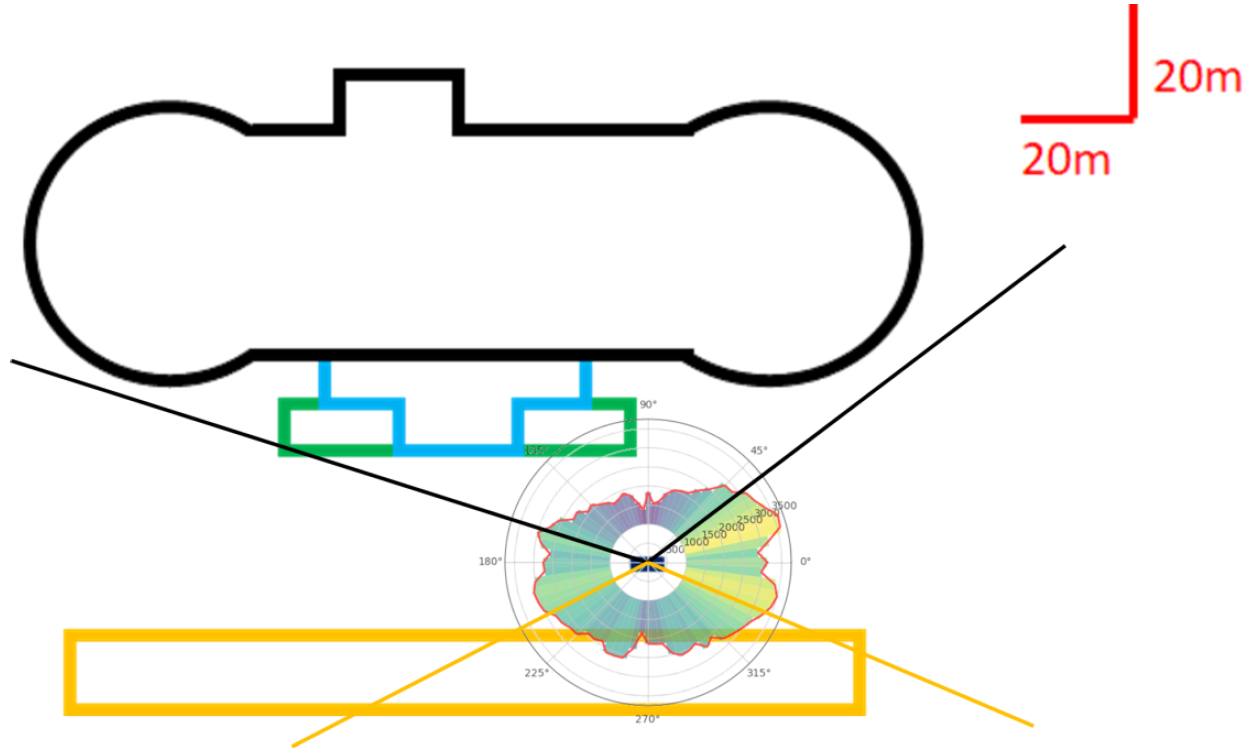
\includegraphics[width=\linewidth]{Chapter5/Figs/Raster/cirOverlayReversedWylfaSlice0-37.5.png}
%  \captionof{figure}{The circular distribution of the $\phi$ from a $\theta$ of 0$^\circ$ 37.5$^\circ$ traced over from google maps and then compared with the documentation given by Wylfa reactor operators. The reactor shadow is now dominated by the main reactor building.} %~can be used as a kind of place holder in latex
%  \label{fig:wylfaTraceAbove52.5}
% \end{figure}

% As can be seen in the data for the Wylfa deployment (figure \ref{fig:pVsTWylfaReversed}) and the Liverpool deployment (figure \ref{fig:pVsTLiverpoolReversed}) the segmentation of the detector dominates the colour map. In figure \ref{fig:pVsTWylfaReversed} for example the distribution pointing towards the sky, towards 90$^\circ \theta$, there is angular bin migration pulling towards the vertical bins at $\phi$s 0$^\circ$, 90$^\circ$, 180$^\circ$, 270$^\circ$. This 2d bin migration in both $\theta$ and $\phi$ is due to the segmentation of the detector. It masks the shadows in the data. In theory it would be possible to use simulated data as a control for both the Liverpool and the Wylfa data sets unfortunately this would also require an understanding of all possible conditions that could cause potential variance. This includes the weather, the noise produced by the reactor at Wylfa, the effect of the height of Brunlow hill at Liverpool and how often double cosmics occur inside the detector. Whilst in theory it would be possible to account for all of those different systematic uncertainties there are still many random factors that could still cause significant differences between the simulation and measured data.
% \\\\ As a result it is more effective to use the Liverpool data as control data for the Wylfa data, providing the Liverpool data is only used as a control above 17.5$^\circ \theta$ to avoid the shadows in the Liverpool data. This technique will still be affected by the difference in data collection techniques between Wylfa and Liverpool namely that Liverpool was switched to a cosmic $\mu$ mode and Liverpool is on Brunlow Hill which will also impact the distribution. However, all other variations will be dived by each other in a ratio plot, figure \ref{fig:wylfaDivLiverpool} shows that the shadows are much more visible once a ratio between the two data sets is taken. The excess and the deficit are roughly analogous to density measurements where an excess ($>$ 1) in figure \ref{fig:wylfaDivLiverpool} can be considered areas of low density and areas in deficit ($<$ 1) can be considered areas of high density. 
% \\\\ Alternative colour maps for figure \ref{fig:wylfaDivLiverpool} can be seen in figure \ref{fig:wylfaToLiverpoolRatioCustomMaps} these custom maps have different pros and cons and ultimately were dropped in favour of the scheme used in figure \ref{fig:wylfaDivLiverpool}. The ``stark'' colour map see in figure  \ref{subFig:wylfaToLiverpoolRatioStarkMap} shows the deficit (attenuation of cosmic $\mu$) caused by the building shadows at wylfa very clearly, however this colour map makes the edges of the shadows seem sharper than is justifiable. The ``sanitised'' rainbow map seen in figure \ref{subFig:wylfaToLiverpoolRatioSanRbMap} shows the edges of the shadows more clearly than \ref{fig:wylfaDivLiverpool} and shows the difference in density between the turbine hall centred at 270$^{\circ}$ and the reactor buildings centred at 90$^{\circ}$ very clearly however it is unclear to colour blind viewers and so was discarded. Both of the alternate colour maps shown in figure \ref{fig:wylfaToLiverpoolRatioCustomMaps} are also unclear in grey scale when compared to \ref{fig:wylfaDivLiverpool}.
   
% \begin{figure}[H]
%  \centering
%  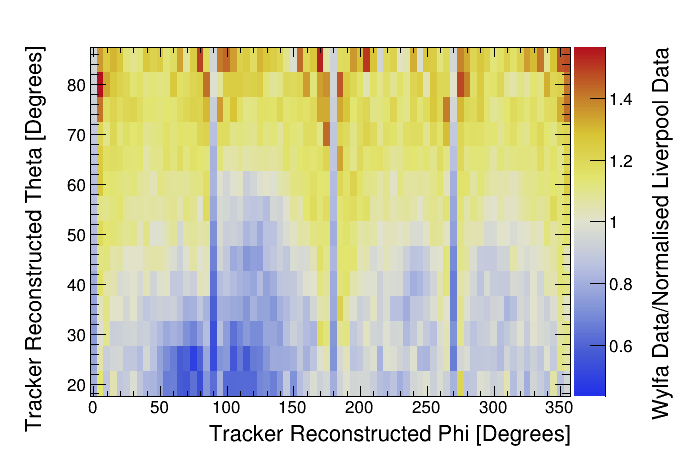
\includegraphics[width=1.0\linewidth]{Chapter5/Figs/Raster/wylfaToLiverpoolRatioDynamic17.5-87.5.png}
%  \captionof{figure}{The ratio of the Wylfa $\theta$ and $\phi$ cosmic muon distribution divided by the Liverpool $\theta$ and $\phi$ cosmic muon distribution. The Liverpool data is normalised to the Wylfa data. The ratio minimum $\sim$ 0.5 represents a deficit (attenuation) of $\sim$ 50\,$\%$. The maximum ratio $\sim$ 1.5 represents an excess of $\sim$ 50\,$\%$.} %~can be used as a kind of place holder in latex
%  \label{fig:wylfaDivLiverpool}
% \end{figure}

% \begin{figure}[H]
% \centering
% \begin{subfigure}{.5\textwidth}
%   \centering
%   \includegraphics[width=\linewidth]{Chapter5/Figs/Raster/WylfaToLiverpoolRatio_starkMap.png}
%   \captionsetup{width=.9\linewidth}
%   \caption{``Stark'' colour map .}
%   \label{subFig:wylfaToLiverpoolRatioStarkMap}
% \end{subfigure}%
% \begin{subfigure}{.5\textwidth}
%   \centering
%   \includegraphics[width=\linewidth]{Chapter5/Figs/Raster/WylfaToLiverpoolRatio_sanRbMap.png}
%   \captionsetup{width=.9\linewidth}
%   \caption{``Sanitised'' rainbow colour map.}
%   \label{subFig:wylfaToLiverpoolRatioSanRbMap}
% \end{subfigure}
% \caption{Alternative colour maps for figure \ref{fig:wylfaDivLiverpool}. }
% \label{fig:wylfaToLiverpoolRatioCustomMaps}
% \end{figure}

% From figure \ref{fig:wylfaDivLiverpool} rough height estimates for the main reactor building and the reactor service buildings seen in figure \ref{fig:wylfaHieghts} can be made. These rough approximations can then be put into the GEANT4 simulation of the detector, this combined with the traces from google maps \hl{show the traces from google maps before this point!!!} allows for the approximations seen in figure \ref{fig:simulatedReactorBuildings}. This is then combined with a realistic redistributed $\theta$ distribution \hl{need to add the redistributed theta stuff} taken from the Wylfa distribution which was taken at sea level. 
% \\\\ The ratio between the simulation with and without the reactor buildings can be seen in figure \ref{fig:simulatedShadowDist} the shadow distribution matches the overall shape of the distribution seen in figure \ref{fig:wylfaDivLiverpool} for the main reactor buildings. However the building heights actually appear to be slightly taller than expected when compared to the measured results, the heights in figure \ref{fig:wylfaDivLiverpool} extend to a maximum of 60$^\circ$ in $\theta$ whereas the heights of the buildings in figure \ref{fig:simulatedShadowDist} extend to 65$^\circ$ in $\theta$. This shows that the simulated heights need to change in order more accurately represent the data and as such round the height estimates down from 40\,m to 35\,m. \hl{need to add in plots with revamped heights in simulation}

% \begin{figure}[H]
%  \centering
%  \includegraphics[width=1.0\linewidth]{Chapter5/Figs/Raster/wyflaHieghtsNew.png}
%  \captionof{figure}{The estimated heights of the reactor buildings, above 32.5$^{\circ}$ the green tower closest to the detector dominates, above 52.5$^{\circ}$ the main reactor building dominates the shadow. \hl{adjust angles and heights}} %~can be used as a kind of place holder in latex
%  \label{fig:wylfaHieghts}
% \end{figure}

% \begin{figure}[H]
% \centering
% \begin{subfigure}{.5\textwidth}
%   \centering
%   \includegraphics[width=0.685\linewidth]{Chapter5/Figs/Raster/reactorBuildingsTopDown.png}
%   \captionsetup{width=.9\linewidth}
%   \caption{Top down perspective of simulated reactor buildings in Geant4.}
%   \label{subFig:simulatedReactorBuildingsTopDown}
% \end{subfigure}%
% \begin{subfigure}{.5\textwidth}
%   \centering
%   \includegraphics[width=\linewidth]{Chapter5/Figs/Raster/reactorBulidingsDepth.png}
%   \captionsetup{width=.9\linewidth}
%   \caption{Side on Perspective of simulated reactor buildings in Geant4.}
%   \label{subFig:simulatedReactorBuildingsDepth}
% \end{subfigure}
% \caption{The reactor buildings simulated in Geant 4 next to the detector which is at the origin.}
% \label{fig:simulatedReactorBuildings}
% \end{figure}


% \begin{figure}[H]
%  \centering
%  \includegraphics[width=0.8\linewidth]{Chapter5/Figs/Raster/reactor100PercentRatio.png}
%  \captionof{figure}{The simulated reactor shadow assuming the heights calculated from figures \ref{fig:wylfaDivLiverpool} and \ref{fig:wylfaHieghts} and assuming that each building is made from 100\,\% concrete. And then the ratio is taken between the simulated data both with and without the reactor shadow present. The building placement is show in figure \ref{fig:simulatedReactorBuildings}.} 
%  \label{fig:simulatedShadowDist}
% \end{figure}

% \section{Cosmic Tracker Uncertainties} \label{sec:CosmicTrackerUncertainties}

% end